% !TeX document-id = {926c0bfa-5bf3-48c1-ab3d-11e1d15aeb22}
% !BIB TS-program = biber
%--------------------
% Packages
% -------------------
\documentclass[11pt,a4paper]{article}
\usepackage[T1]{fontenc}
\usepackage{mathptmx} % Use Times Font
\usepackage{times}
\usepackage{amsmath}
\usepackage[UKenglish]{babel}
\usepackage[style=authoryear,backend=biber,uniquename=false,maxnames=2,minnames=1,natbib=true,eprint=false,url=true,isbn=false,date=year]{biblatex} %Imports biblatex package
\usepackage{csquotes}
\usepackage{placeins}
\usepackage{afterpage}
\addbibresource{ref.bib}
\usepackage[pdftex]{graphicx} % Required for including pictures
\usepackage[pdftex,linkcolor=black,pdfborder={0 0 0}]{hyperref} % Format links for pdf
\usepackage{calc} % To reset the counter in the document after title page
\usepackage{enumitem} % Includes lists
\usepackage{booktabs}
\frenchspacing % No double spacing between sentences
\linespread{1.2} % Set linespace
\usepackage[a4paper, lmargin=0.1666\paperwidth, rmargin=0.1666\paperwidth, tmargin=0.1111\paperheight, bmargin=0.1111\paperheight]{geometry} %margins
%\usepackage{parskip}
\DeclareGraphicsExtensions{.pdf,.png}
\usepackage[all]{nowidow} % Tries to remove widows
\usepackage[protrusion=true,expansion=true]{microtype} % Improves typography, load after fontpackage is selected




%-----------------------
% Set pdf information and add title, fill in the fields
%-----------------------

\title{Attribution of extreme precipitation related to a fatal Derailment  near Carmont, Scotland}
\author{Simon F. B. Tett\thanks{School of Geosciences, University of Edinburgh, Edinburgh EH9 3JW, UK} \thanks{ARC Centre of Excellence for Climate Extremes,
University of New South Wales,
Sydney, NSW 2052 Australia}
	\and 
Chris Long\thanks{School of Physics and Astronomy, University of Edinburgh, Edinburgh EH9 3JZ, UK}
\and 
Simon J. Brown\thanks{Met Office Hadley Centre, Fitzroy Road, Exeter, EX1 3PB, UK}}


%-----------------------
% Begin document
%-----------------------

\begin{document}
	
\maketitle

\graphicspath{{../figures/}}


\begin{abstract}
	A derailment on 2020-08-12 near Carmont, Scotland resulted in the death of three people and the injury of the other 6 people on the train. The cause of the derailment was gravel washed onto the tracks due to heavy rain and an improperly built drain.  The heavy rainfall near the derailment site lasted about 4 hours, with a large burst of  rain just prior to the derailment. The rainfall event was heavy with return  periods between 1-in-20  and 1-in-40 summers. Simple theory suggests that extreme precipitation should increase with changes in saturated humidity (Clausius-Clapyron; CC). The UK's Convective Permitting Model suggests, that extreme hourly rainfall near Carmont changes at  about 1.5 x CC rates while extreme four hourly rates increases below  CC rates. This leads to an increased probability, relative to late 19th century conditions,  of hourly (4-hourly) extremes similar to that which occurred near the derailment by about 20 (15)\% with a further frequency increase of about 20 (15)  \% for such events in a +2C warmer world. Some characteristics of the simulated extreme rain evaluate well against radar values, but the  simulated rainfall is about 20-30\% larger than the radar rainfall. This likely reflects shortcomings in  radar  calibration of extreme rainfall though poor  model performance is also possible. 
\end{abstract}



\section{Introduction}
\label{sect:Intro}

On August 12th 2020 a passenger train running from Aberdeen to Glasgow derailed at Carmont near Stonehaven. The train was lightly loaded due to COVID restrictions. Even so,  three people died and the remaining six people on the train  were injured. The proximate cause of the derailment was gravel being washed out of a drain with contemporary radar estimates of 1km x 1km resolution rain as 51.5 mm of rain falling between 05:50 to 09:00  estimated at around a 1-in-a-100 year event\parencite{carmontReport2024}. The drain should have been able to deal with that volume of water, but because the drain had not been built to design requirements, gravel and other debris was washed out of it and onto the tracks. This in turn caused the derailment. In the aftermath of the derailment, the UK Government commissioned a report to examine the resilience of the UK's rail infrastructure\parencite{NR_DfT_2021}. It reported that the signal of climate change is becoming more significant and also examined the impacts of future climate change  on rail infrastructure.


 Serious accidents often require several things to go wrong. In the case of Carmont derailment,   both a drain constructed not to specification and extreme rainfall were required. This paper focuses on the rainfall component of the accident. It develops methodology to estimate, from radar data, the return period of the radar rain. Then uses convective permitting model (CPM) simulations to estimate how climate change (largely anthropogenic) has changed the distribution of extreme precipitation at Carmont. Finally, we  provide an  attribution assessment for the extreme rainfall and estimate extreme rainfall probability distributions in a future warmer world. 
 
 
 In the language of \cite{Shepherd2016} we are carrying out a ``risk-based'' attribution.  The first of these were carried out by \cite{Stott_2004} who examined the 2003 heat wave defining the event as a seasonal temperature anomaly. \cite{Otto2012russian} examined the 2010 Russian heatwave with a focus on trying to reconcile different claims on the relative impact of natural variability and anthropogenic climate change. They resolved the discrepancy by noting much of the intensity change was driven by the natural circulation but the changing  occurrence frequency was largely driven by anthropogenic forcing. Attribution of seasonal scale rainfall extremes (for example \cite{li2018yangtze,christidis2022wetUK}) have shown modest increases in probability.  Limited analysis of daily-monthly  extremes \parencite{Pei2022precip,Kawase2022japan_rain,Kawase2020rain,tradowsky2023w_europe_rain} also suggests a small anthropogenic influence.  Some studies have attempted to attribute daily extremes to anthropogenic forcings (for example  \cite{Eden2018dutchrain,Tozer2020tas_rain,Li2022typhoon_rain,Zhang2020rainfall}) though only \cite{Li2022typhoon_rain,Zhang2020rainfall}  found an unambiguous change in daily extreme rainfall due to human influences. 

Theory\parencite{allen02insight} suggests that extreme rainfall occurs when the entire column of atmospheric water precipitates. This, in turn,  suggests that extreme precipitation increases fractionally at the same rate as saturated humidity, or for fixed atmospheric pressure, saturated vapour pressure (Clausius-Clapeyron; CC). This is about 7\%/K. However,  studies suggest that sub-daily extreme rainfall  could increase  at rates  up to twice CC\parencite{fowler2021rainfall_extremes} with a clear signal in both observations and CPM relating contemporaneous dew-point temperature to extreme rainfall. 
 

The last IPCC report\parencite{Seneviratne2021ippcc_chapter_extremes} reported on the lack of systematic analysis of long-term trend in sub-daily extreme precipitation at global scales (Sect 11.4). Though, it did report on regional studies that found intensification at those scales.  There has  been an extremely limited number of studies that attempted to attribute changes in sub-daily extreme rainfall, with none reported in \cite{Seneviratne2021ippcc_chapter_extremes}.   \cite{mishra2023landslide}  used a  CPM to simulate a 2009 storm with contemporary and  pre-industrial conditions and found that changes in three-hourly extremes had increased the frequency of landslides by about 10\%. \cite{matte2022cloudburst}  used a CPM to investigate a cloudburst  event in July 2011 that impacted  Copenhagen. They found an increase in the probability of unprecedented precipitation.  \cite{Reed2022,Reed2021dorian_extreme_rain} examined North Atlantic hurricanes  using a CPM and found that climate change had increased extreme 3-hourly rainfall by 11\% and, for Hurricane Dorian by 8-18\%. \cite{tett2023edinburgh} used radar and CPM data to estimate the change in probability of a ``cloudburst'' event at Edinburgh Castle. They also examined the impact on the Castle.  This study develops the methodology they used to estimate the probability changes and evaluates the CPM. 

 
 
The rest of this paper is laid out as follows. We first describe the data we use,  then describe the event and its impact,  describe our methodology, show results and, finally,  conclude. 

\section{Data}
\label{sect:data}

\subsection{Radar rainfall}
\cite{saltikoff2019radar_climate} suggested that radar data is now useful for quantitative climate studies.  Radar rainfall for the United Kingdom is available from April 2004 to near-present\parencite{radar_data} from the Nimrod\footnote{This is not an acronym.} archive. The UK's Met Office process for conversion of radar reflectivity to quantitative precipitation estimates is described by \cite{harrison2000nimrod,Harrison2012,procedings:harrison15radarnet}. The rainfall data is available  as  1km 5-minute and 5km 15-minute  averages though may underestimate extreme precipitation\parencite{harrison2000nimrod}. The two closest radar stations to the rail accident are Munduff Hill and Hill of Dudwick. Both stations are in eastern Scotland but Munduff Hill opened in 2008. So,  we use radar rainfall  data from  2008-01-01 to 2023-12-31. 


\subsection{Convective Permitting Model}
 As part of the UKCP18 project a 12 member ensemble of Convective Permitting Model (CPM) simulations, at a resolution of 2.2 km, was carried out\parencite{kendon2023uk_cpm} which showed intensification of hourly extreme rainfall, particularly in the northern part of the UK. The CPM had 70 vertical levels and the resolution reduced from 2.2km over much of the domain to 4.4 km at the boundaries. See \cite{art:fosser20} for more details on the CPM configuration and justification for choices. Each CPM ensemble member had different boundary conditions and was ran from 1980 to 2080.  The boundary conditions  are from 12km resolution regional atmospheric models which are driven by  60km global coupled models. Daily average sea-surface temperatures (and sea-ice concentrations) used in the CPM and regional model simulations were taken from the global models. The global models differ in their parameter choices. The CPM ensemble, however, due to the advection scheme employed, includes occurrences of unphysical heavy rainfall in certain situations.  Data, after filtering out such rainfall, are used to estimate how extreme rainfall changes with temperature. 

\subsection{Additional data}
We also use the observed Central England Temperature (CET) record\parencite{parker92cet}. We compute a CPM simulated equivalent from the weighted average from the cells closest to the 4 weather stations used in \cite{parker92cet}.  

\section{Carmont Event}

In this section, we describe the Carmont rainfall event and its impact. We then use that to determine what the event is for subsequent analysis. Fig~\ref{fig:carmont_geog_group}(a) shows the topography and location of various places in North-East Scotland, with an inset map showing Great Britain and some of Ireland. The railway from Aberdeen runs largely along the coast, except for a deviation inland between Montrose and Stonehaven.  The dominant topographic feature is the Grampians,  which is an extensive area greater than 500m above sea level. The area of interest has, from 2008, two radar stations with much of the region within 60km of one radar station and  all the region within 120km of a radar station and most within 120 km of two radar stations. 

  The event starts in the evening of 2020-08-11 and ends the next day. At 12:00 UTC on the 11th there is high pressure over Great Britain with weak south-westerly airflow over Scotland and a convergence line running from the Lake district (North West England) to the North of Scotland\parencite{pritchard2020weather}. By the 12th, the convergence line has moved to the west into the North Sea, though NE Scotland was still in an SW flow. 

On  the evening of the 11th  a large thunderstorm initiated in the Scottish Borders and over the next few hours propagated northwards, eventually heading out to sea by early morning on the 12th\parencite{Kendon2020thunderstrorms_report}. On its way it caused extensive flooding and damage in the eastern part of the Central Belt of Scotland\parencite{SEPA2020report_floods,kendon2021ukclimate} and  Stonehaven. The Stonehaven flooding was largely due to surface water with a small contribution from the river Carron. \cite{SEPA2020report_floods} assessed the rainfall as  extreme and rare. Over the Leven hills in Fife the rainfall was sufficiently extreme to produce multiple land slides -- the first such event there since the early 20th century\parencite{Kirkbride2021}.  Stations at Aviemore and Dyce Airport\parencite{pritchard2020weather} reported monthly extremes of 9.6 and 26.8 mm.

\cite{carmontReport2024} (RAIB from hereon) reported that on the morning of the 12th, after some hours of extreme rainfall, the 06:38 south-bound service from Aberdeen to Glasgow travelled past Carmont, between Stonehaven and Montrose (para S1). Due to a landslip reported ahead, the train reversed to return to Stonehaven. On this journey, the train impacted debris washed out from a drain. The train derailed, resulting in three fatalities, with the other six passengers being injured (RAIB para S1).The train was travelling just below the normal line speed of 117 km/h (RAIB para S2). Extreme rainfall caused flows of surface water that the drain was unable to safely manage. This failure was because the drain was not built to specification (RAIB paras S13-S16) and that railway operations did not fully account for the risks posed by the extreme rainfall (paras S29-S40). 1km radar rainfall estimates for the Carmont Drain site are that 51.5 mm fell between 05:50 and about 09:00 with return periods of about 1 in a hundred years for a three-hour accumulation (RAIB para S10.)

Due to the COVID-19 pandemic, the train had an extremely low loading of only nine people compared to its capacity of 300. Under normal circumstances, between 25 and 50 passengers would have been on the train. With this larger passenger load, the derailment would have likely resulted in a far higher number of casualties and injuries (RAIB para. S78). 

The derailment occurred to the south-west of where the train crosses the Carron Water (RAIB para S1), with the train coming to a halt a few meters after this bridge (Fig.~\ref{fig:carmont_geog_group}(a)).  RAIB commissioned some detailed modelling of water flow into the drain, concluding that flows into the gully being drained occurred in about an hour (RAIB figure 43; para. 104). 


Radar rainfall maxima 4-hour accumulations (Rx4h) for JJA 2020 (Fig.~\ref{fig:carmont_geog_group}(c)) show two small regions  where rainfall is greater than 50 mm. One in the SW of the domain and another along the railway line between Montrose and Stonehaven. Fig.~\ref{fig:carmont_geog_group}(d) shows that these two extrema occurred on the 12th. Looking at radar rainfall on the 12th at Carmont Drain (Fig.~\ref{fig:aug2020_rain}) shows that, for both the 1km and 5 km datasets, the rainfall fell over a period of about 4 hours. For the 1km rainfall, half the accumulated rainfall fell in about an hour.  Resampling the data to hourly data we see that almost all the rain fell in three hours with a substantial contribution from the last hour. Thus, we consider both Rx1h and Rx4h from hereon. The drain for which gravel washout was the proximate cause of the derailment drains the hill to the west of the track (RAIB paras S1-S5) and so we focus subsequent analysis on that location (``Carmont Drain'').

\section{Methods}
In this section, we describe the methods used in the analysis. They are split into processing of the Convective Permitting Model to remove unphysical rain events  and computation of maxima, how the radar is analysed, definition of an event for analysis and, finally, how probabilities of exceeding thresholds are computed. 

All analysis uses a 150x150 km square region centred on Carmont Drain (2.327W, 56.952N) shown in Fig.~\ref{fig:carmont_geog_group}c. As the derailment happened in August, we restrict our analysis to June-July-August (``Summer'' in Scotland).  We generally present summer  maximum accumulations of rainfall from both models and Radar rainfall over N hours. We term these RxNh where N is the number of hours over which the accumulation was computed. 

\subsection{CPM data processing}
We use the full 100 year, 12 member ensemble data. The UK's CPM outputs hourly average rainfall on UTC hours, with a nominal timestamp of HH:30. 

A Semi-Lagrangian advection scheme is employed in the CPM which does not intrinsically conserve the quantities it advects. This has the undesired consequence that in certain rare conditions a moisture anomaly in a single cell or  an one cell wide row or column aligned with the grid can persist in spite of moisture being advected out of the cells. This results in a limitless source of moisture, sometimes referred to as an ''eternal fountain''.  This limitless moisture source can result in very high rainfall rates and accumulations.  These ''fountain'' events can populate a significant proportion of the highest rainfall rates produced by the CPM and have the potential to distort the climatology of extreme rainfall.  As might be expected, this phenomenon is more prevalent during conditions where there is more convection, thus biasing the occurrence of such events to being over the sea during winter, land during the summer and a mixture during spring and autumn.

To address this issue, a filtering and filling procedure is employed.  Firstly, unphysical rain is identified by applying small convolution kernels across the hourly rainfall fields that are constructed to return high values when aligned with the spatial characteristics of the fountain events (isolated high values, horizontal or vertical bars).  Appropriate thresholds to identify "bad" rain from "good" was determined by eye.  Secondly, once "bad" rainfall has been identified, it was set missing. 

All filtered CPM hourly mean rainfall was then aggregated to 4.4 km resolution by simple averaging over 4 cells.  2, 4  and 8 hour rolling averages were then computed from the hourly-mean data. For each grid point and rolling period (including the original data),  the seasonal hourly maximum and date/time of maxima was computed for all seasons and years in the ensemble. We focus on the filtered data but  explore sensitivity to filtering by showing some results from unfiltered (``Raw'') model data.

Regional temperatures and precipitation were computed from seasonal-average values over the 150x150 km region. Land versions were computed using only land cells. Saturated Vapour Pressure (SVP) was computed from the daily mean temperature and the improved Magnus relationship (Eqn~3 of \cite{Huang2018SVP}) and then seasonally averaged.

\subsection{Radar analysis}
We aggregate both the  1km 5-minute and 5km 15-minute rainfall data to UTC hourly means, requiring, for any day, data from at least 6  unique hours. As a crude form of quality control, data was set missing if the rain rate was greater than 400 mm/hour.  The 1km data was then aggregated to 4 (1km-c4) and 5km (1km-c5) resolution by averaging 16 or 25 cells, respectively. Data was then rolling accumulated to 1, 2, \&  4 hours. Seasonal maxima, for each accumulation period,  and the time/date of the  maximum were computed for each rolling period and at each gridpoint. This gives four summary radar datasets (1km, 5km,  1km-c4 and  1km-c5). Much of our analysis focuses on the 1km dataset, with the  other three datasets used to compare with the CPM simulations. 

Radar datasets can suffer from various artefacts \parencite{Overeem2023euradclim}.
For the Carmont region, both the summer mean rainfall and the median of the 1-hour maximum rainfall in summer are largely free of artefacts (Fig~\ref{fig:radar_jja}). There are two artefacts associated with the Munduff hill site on the southern end of the domain, visible in the summer mean rain. There are also a few localised areas over the North Sea which may be radar artefacts.  Beyond these, the clearest signal is a strong land/sea contrast in both the mean and maximum rain. Overall, the radar data appears to be adequate for our purposes.  

\subsection{Event Definition}


To accurately estimate distributions, and their uncertainness,  requires a independent values, but extreme rainfall in two locations close in space and time are likely from the same  system and so are not independent.  We crudely deal with this by defining an event  as all summer maxima  occurring on the same UTC day over land in the Carmont region. Figure~\ref{fig:carmont_geog_group}(c) shows Rx4h  for summer 2020 and  those Rx4h  that occurred on  August 12th  from the 1km radar dataset. This event had an area of about 6000 km$^2$ which makes it a rare large event. There is no obvious  reason why event size and rainfall intensity should be related to size so we believe this is not a selection effect.  Quantiles, with respect to rainfall accumulation,  are computed, for each event,  at values from $0$ to $1$ in steps of $0.05$. As well as the accumulation the position, time, and topographic height of the nearest matching cell are computed. The  number of cells, and so area, of the event is also recorded.  Events are computed independently for Rx1, Rx2h and Rx4h. An event is then represented by the seasonal maximum rainfall accumulation at 21  quantiles  with some additional data. 

These events are computed for  16 years of radar data and  the CPM data. 
To compute a distribution for the whole land region, for the 15 years of radar data, we pool all radar events and  randomly select, for each event, a single quantile. A GEV is then fit to this pooled data \parencite{gilleland2016extremes} with the data weighted by the number of cells (or area)  in the event. This process was repeated 1000 times and the fit parameters and covariances averaged. For the 1km (5km) dataset we have 703 (421) and 576 (326)  events for 1-hour and 4-hour accumulations.   In doing this we are assuming we can pool in space and time to estimate the distribution of maximum events. 

\subsection{CPM Statistical Models}

%\cite{fowler2021rainfall_extremes} argues that extreme precipitation is related to concurrent dew point temperature (rather than temperature) as above a dry bulb of  25C  extreme precipitation falls with temperature.  However, \cite{Visser2021hook_precipitation} found, for Australian rainfall stations, that this ``hook'' was explained by changes in rainfall event duration while \cite{Seneviratne2021ippcc_chapter_extremes} found that the contemporaneous dew-point/extreme rainfall relationship was not very robust. 

To examine risk changes we  estimate how the extreme distribution changes with seasonal temperature by fitting statistical models to the CPM summer extremes. We use the extRemes R library\parencite{gilleland2016extremes} to fit a generalised extreme value distribution\parencite{Coles_2001} with covariates on the location  ($\mu$) and scale  ($\sigma$) parameters, and a fixed shape ($\zeta$).  From the this fit, we can estimate probabilities of extremes at specified covariate values.  We consider several different statistical models:
\begin{description}
	\item[No Covariate] Fixed GEV distribution. 
	\item[C] Use JJA mean Central England Temperature (CET;\cite{parker92cet}) as a covariate.
	%%\item[CET+CET$^2$] Use both CET and CET$^2$ as covariates. This model would be able to crudely represent any non-linearities in the relationship between temperature and extreme precipitation. 
	\item[T] Use average summer temperature in the Carmont region as a covariate.
	\item[S] Use average summer saturated vapour pressure (SVP) in the Carmont region as a covariate. 
\end{description}
We also use 2nd order  models for CET ($C+C^2$), Regional temperature ($T+T^2$) and SVP ($S+S^2$). These models are able to crudely represent any non-linearities in the relationship between temperature and extreme precipitation. 

 We  use the Akaike information criteria\parencite{akaike74aic} to compare different statistical models. To test for fit adequacy we use the  Kolmogorov-Smirnoff (K-S) test. The K-S test is not a particularly powerful test\parencite{stephens74fit}, but alternatives are not very suitable for the GEV. However, to apply the K-S test we need to normalise the GEV so all data ($x(t)$) is transformed:
\begin{equation}
	x'(t_i)=\frac{x(t_i)-\mu(t_i)}{\sigma(t_i)}
\end{equation}
where $\mu(t)$ and $\sigma(t)$ are the location and scale parameters at time $t$ and ensemble member $i$ computed from the covariate fits. 
If the fit is adequate then $x'$ should be distributed as a GEV with $\mu=0, \sigma=1\ \text{and shape}=\zeta$. We test for adequacy by averaging the K-S test values over the Carmont region. On the basis of this (Table~\ref{tab:ks}) all statistical models perform adequately for all RxNh values.  


Before examining  the statistical summaries, we examine scatter plots between CET and the other variables, as well as regional temperature vs SVP (Fig.~\ref{fig:cet_scatter}). This shows that the CPMs have large CET biases for 2008-2013, which depends on the ensemble (Fig.~\ref{fig:cet_scatter}a) ranging from -0.5$^\circ$C to +2.5$^\circ$C. The CPM ensemble-average  is $17.2^\circ$C which is about a degree larger than the observed $16.1^\circ$C. Average temperatures for 2065-2080 range from $18.7^\circ$C to $22.2^\circ$C, depending on the ensemble member,  with an ensemble-average of  $20.8^\circ$C.

Our use of the CPM is to compute the sensitivity of CPM GEV parameters to temperature and then apply those to the radar rainfall distributions. Thus, our analysis is not sensitive to model bias as long as the bias does not impact the parameter sensitivity.  Simulated Carmont regional temperature (Fig.~\ref{fig:cet_scatter}(a)) is strongly correlated with CET and warms at $78\pm1$\% of CET changes. This presumably arises from the sea warming less than the land and a more maritime climate over NE Scotland than in the CET region. Regional SVP also correlates well with CET (Fig.~\ref{fig:cet_scatter}(b)) and increases at $5.70\pm 0.04$\% per degree CET warming. Thus, Clausius-Clapyron would suggest the extreme precipitation should increase by 5.7\% per degree of \textit{CET} smaller than the local temperature relationship. Regional  average precipitation falls with temperature, though there is considerable variability and so the R$^2$ is small.  Regional SVP and temperature (Fig~\ref{fig:cet_scatter}d) are strongly correlated, though at low or high temperatures there is a systematic deviation from the linear fit as the exponential behaviour of SVP becomes apparent. The \textit{local} relationship between temperature and SVP at $6.85\%^\circ\text{C}^{-1}$ is larger than between CET and local SVP.  
 
We fit several different statistical models to the simulated  extreme event data. Based on the AIC we conclude that adding covariates, that capture climate change, improves the AIC (Table~\ref{tab:aic}) with the best model one that uses regional temperature. There is little improvement, or occasionally, some worsening when using a 2nd order model, suggesting that non-linear effects are not important. Using land only covariates makes things worse, suggesting that extreme rainfall is being controlled by large-scale temperatures.  The CET covariate performs worse than  regional  temperatures or regional SVP. Even though it is worse, we prefer to use it as the CET record covers the late 19th century, allowing us to compare RxNh probabilities to  late 19th century values.

\subsection{Attribution and uncertainty analysis}

To give estimated extreme distributions for  CET values we  scale the radar fit shape and location parameters by the fractional changes, relative to 2008-2023, from the CPM covariate fits with respect to CET.  \cite{tett2023edinburgh} motivates this as  GEV intensity scales with fractional changes in parameters\parencite{Coles_2001}. If precipitation extremes scale like local Clausius-Clapeyron (about 7\%/degree warming) then the scale and location values would also change by about 7\%/degree local warming.  For the location ($\mu$), scale ($\sigma$) and shape ($\zeta$) parameters, this is:

\begin{equation}\label{eq:gev_params}
\begin{aligned}
\mu(C) =& \mu_r \left( 1+  \frac{(C-C_t)}{\mu_m} \frac{d\mu_m}{dC_m}\right)\\
\sigma(C) =& \sigma_r\left ( 1+  \frac{(C-C_t)}{\sigma_m}  \frac{d\sigma_m}{dC_m}\right)\\
\zeta(C)=&\zeta_r
\end{aligned}
\end{equation}
where subscript $r$ (m) are radar (CPM) values, $C$ is the JJA Central England Temperature averaged over the time of interest, and $C_t$ is the average JJA CET for ``today'' (2008-2023). The model parameter values all come from extreme-value fits, using a CET covariate, to the CPM data. These can, in theory, be used for any CET JJA value though it would be unwise to extend this relationship outside the simulated CET range (about $14^\circ$C -- $23^\circ$C; Fig~\ref{fig:cet_scatter}b).   

We compute, for example, the pre-industrial distribution from  the  JJA 1850-1899 CET difference from 2008-2023  which gives, from equation~\ref{eq:gev_params}, the GEV parameters. Focusing  on Rx1h when 1850-1899 JJA CET is $0.92^\circ$ cooler than 2008-2023, then the estimated location parameter is:
 \begin{align*}
 \mu(1850-1899) =& \mu_r \left( 1 - \frac{0.91}{\mu_m} \frac{d\mu_m}{dC_m}\right) \\
   =&  \mu_r \left( 1 - \frac{0.91}{8.30} 0.33\right)\\
  \mu(1850-1899) = &0.96\mu_r
 	\end{align*}
 
 Similarly the estimated scale parameter is:
 
 \begin{align*}
	\sigma(1850-1899) =& \sigma_r \left( 1 - \frac{0.91}{\sigma_m} \frac{d\sigma_m}{dC_m}\right) \\
	=&  \sigma_r \left( 1 -  \frac{0.91}{3.32} 0.31\right)\\
	\sigma(1850-1899) = &0.92\sigma_r
\end{align*}

 From the estimated parameters, we compute the intensity of  extreme values from the survival function and probabilities of exceeding values  from the  inverse survival function. We compute return period from one over probability of specified exceeding threshold. We compute probability (PR) and intensity (IR) ratios from these distributions, relative to pre-industrial values (PI;1850-1899) for a range of radar rainfalls and return periods by comparing values for average CET values for 1980-1990, 2008-2023 and global warming of $+2^\circ$C corresponding to a JJA CET of $17.09^\circ$C (PI$+1.84^\circ$C or$+0.96^\circ$C warmer than 2008-2023; \cite{tett2023edinburgh}). As (see later) the CPM changes are quite noisy, we average the parameters and covariance over a 5x5 block (approximately 22x22 km) centred on Carmont drain.

To compute radar uncertainties, we use the parameter covariance  estimates \parencite{gilleland2016extremes}. Uncertainties in the CPM fits are computed by sampling with replacement\parencite{Efron1994bootstrap} in time and ensemble member  to generate 100 realisations. The parameter covariance matrix is then computed from these samples. Uncertainties in the CPM adjusted distribution parameters are done by generating 1000 realisations of radar and CPM parameters from thier covariance matrices and then  combining them to give 1000 parameter-set realisations. PR and IR values are computed and 5-95\% ranges computed from these 1000 realisations. 

\section{Results}

In this section, we present our results. We start by looking at the CPM estimate of extremes in the current climate, compare the radar rainfall with the CPM rain and finally examine the change in probability and intensity ratios. 
\subsection{CPM Behaviour}
We focus on the 1-in-hundred year event for Rx1h and Rx4h accumulations for the  2008-2023 average observed CET temperatures. Averaged over the  ensembles the CPM is about 1 degree too warm (Fig.~\ref{fig:cet_scatter}a), so by using observed CET to compute the parameters we are crudely bias correcting the model simulations. A clear signal in Rx1h return values (Figure~\ref{fig:map_intensity}(a)) is a strong land/sea contrast, with oceanic values at least 15\% lower than Carmont Drain.  Over almost all  land points return values are within 15\% of the Carmont Drain values. Exceptions are near the coast in the south and parts of the Grampians  and in the NE of the region. Rx4h  return values are less variable (Figure~\ref{fig:map_intensity}(b)) than Rx1h though some land/sea contrast is apparent.  

If the CPM is accurate then the relatively small range ($\pm$15\%) for both Rx1h and Rx4h  return values suggests that spatial variability, over land,  in extreme rain is not large.  Thus, poooling over space and time for the observed radar rainfall is appropriate. 


Considering the fractional changes in the intensity of the 1-in-100 year per degree CET warming (Figure~\ref{fig:map_intensity}(c \& d)). For Rx1h almost all the region shows super CC behaviour (increases in intensity by more than 5.7\% per degree CET increase) with a strong but noisy,  geographical signal.  Changes of 12\% or larger occur over the Grampians, with the weakest changes occurring over the sea south of 57N. In contrast, Rx4h shows a  more muted geographical signal with no strong land/sea contrast and much of the region, including Carmont Drain, shows intensity changes that are less than CC.  Thus, even at very extreme values we are likely seeing a mixture of dynamical and thermodynamic  changes leading to  strong geographical patterns in  intensity per degree warming.

\subsection{Event return periods}
From the radar data, we can estimate return periods (and uncertainties). We examine both 1km and the three near 5-km datasets for both Rx1h and Rx4h (Fig~\ref{fig:radar_rtn_prd}). For the 1km radar, we estimate the rain associated with the derailment is about a 1-in-20 (40) year event for Rx1h (Rx4h). Uncertainties for both time periods are small reflecting the large number of events. For the three 5km datasets, return periods are more uncertain and dataset dependant. The Rx1h event varies between a 1-in-15 year event to a 1-in-50 year event, while the Rx4h accumulation ranges from a 1-in-50 to a 1-in-150 year event. Uncertainties even for an individual dataset are larger in the 5km dataset than in the 1km dataset reflecting that, at all accumulation times, the 1km dataset has about twice as many events/year as the  5km dataset does (Table~\ref{tab:event_stats}).

Looking at maps of return period for the 2022-08-12 event. For 1km Rx1h (Figure~\ref{fig:map_rtn_prd}(a)) the return periods are, for both the 1km and 5km datasets (Figure~\ref{fig:map_rtn_prd}(b)) over  for much of the event, not very large at around 10-20 summers. However,  to the north of the derailment there is a small region, in both radar datasets, where return periods are about 100 summers.   For Rx4h (Figure~\ref{fig:map_rtn_prd})(c-d)) return periods are larger with a region of long return periods along the railway line where it runs inland. This more apparent in the 5km dataset than in the noisier 1km data. Also, apparent are long return periods at around 3.25W, 56.6N (north of the radar station at Munduff hill). Both of these regions of long return period correspond to the Rx4h accumulations of more than 50mm shown in Figure~\ref{fig:carmont_geog_group}(d). 

\subsection{Comparison between Radar and  CPM}

Table~\ref{tab:max_rain} shows the median Carmont Region RxNh values from the raw and filtered CPM data, and from three roughly 5km radar datasets.
 The effect of filtering is to reduce the median RxNh by 3-4\% with a larger fractional reduction at Rx1h than at Rx4h.  All  radar datasets are less intense than the CPM  with the 5km radar being about 10-15\% smaller than the filtered CPM data.  However, it could be that the radar data is underestimating extremes.
 
 We can also compute events from the CPM data and compare with the near 5km datasets. We compare the number of events per year and the area size across the datasets (Table~\ref{tab:event_stats}). Given the event definition, then the mean area times events/year should be land area times number of years, and is fixed. For all radar and CPM datasets, as the accumulation period increases then area increases (and count decreases). The CPM has smaller, and so more, events than the radar datasets. 
 
  We carry out a qualitative comparison between events in  CPM and radar datasets for 2008-2023 (Figure~\ref{fig:kde_smooth_events}) focusing on the Rx1h and Rx4h results for the 50\% event quantile values. 
  For Rx1h distributions of day-hour, event area and height are qualitatively similar  (Figure~\ref{fig:kde_smooth_events}(a-c)) with all datasets showing day-hour peaks at about 16:00 UTC, event size density dropping rapidly from about 250 km$^2$ and peak density for height of maxima at about 100 m.
   The height distributions for both radar and CPM are very similar to that in the 5km topography dataset, suggesting that the location of the quantiles within events are largely  randomly distributed across the region. 
    For both the radar and model heights, densities  at around 100m are somewhat larger than expected from the topography with lower densities, than expected from the topography, at heights above 500m. 
    There are differences with the model datasets have a slightly smaller peak at 16:00 than the radar datasets have, while the CPM has more extreme rainfall in the early morning than does the radar. The largest difference in the event size distribution is the large dip at around 20km$^2$ seen in the CPM but not in the radar compensated, to some extent, by the overabundance, in the CPM, for event sizes of about 10km. We suspect this is due to ``grid-point storms'' in the CPM which are unphysical. 
     Examining the rain distribution (Figure~\ref{fig:kde_smooth_events}(d)) then, relative to the radar data, the CPM distribution is both more intense and broader with some sensitivity to filtering.  Rx4h (Figure~\ref{fig:kde_smooth_events}(e-h) shows similar behaviour to Rx1h though the day-hour of the maximum rainfall shows bigger differences in the early morning between radar and CPM than Rx1h does, and the CPM generates more rainfall maxima between 600-900m than the radar shows.  Simulated Rx4h, is still intense and too broad compared to the radar datasets. 

\subsection{Attribution}
\label{subsect:attribution}
We now report on our attribution findings. We present these in terms of probability ratio (PR) and  Intensity Change (IC) expressed relative to pre-industrial values (1850-1899). The former tells how much the probability, or frequency, of a given radar rainfall has increased, while the latter tells us how the intensity of a fixed  return period has changed. We express both as \% and consider a range of rainfall accumulations and return periods. We focus on 1km and 5km radar PRs for Rx1h and Rx4 (recall that radar distributions are adjusted by CPM fractional changes).  For IC we only consider 1km as results depend only on return period.  We consider 1980-89, 2008-23, and following \cite{tett2023edinburgh}, a +2C world (which corresponds to a CET of $17.1 \pm 0.06 ^\circ$C.  

Beginning with the Rx1h results (Figure~\ref{fig:intense_prob_ratios}(a-c)) then PR's, for the Carmont rain values of August 2020,  were 104 (median) (104-104; 5-95\%) \% in the 1980s -- a relatively small increase relative to PI. All values are rounded to the nearest \%, with median and 5-95\% values reported. For 2008-2023 they have reached  119 (119-120)\% -- so a 1-in-20-year event in the late 19th Century is now, if the CPM is correct, a 1-in-17 year event.  And should the world warm by $2^\circ$C then PRs are about 141 (138-144)\% for the Carmont rain -- so a 1-in-20 year event in the PI world is now a 1-in-14-year event. The 5km Rx1h PRs are slightly larger than the 1km Rx1h results, though the Carmont values are very similar. Intensity changes for Rx1H are larger than Clausius-Clapeyron across all return periods, with the +2C world having intensity increases of about 14.5 (13.5-15.5) \% for Carmont rain return periods. The unfiltered (``Raw'') CPM data  shows slightly larger PR and IC values than the filtered data.

For Rx4h  (Figure~\ref{fig:intense_prob_ratios}(d-f)) PRs and ICs are smaller than  Rx1h for both 1km and 5km resolutions. For the Carmont 1km  August 20202 rain, then PRs for 2008-2023 (``today'') is about  113 (112-114)\% and increases to 128 (125-131)\% in the potential +2C world. PRs for the 5km radar rain are a bit larger.  Changes in intensity are below Clausius-Clapeyron  up to return periods of 200 summers  (Figure~\ref{fig:intense_prob_ratios}(f)).  There is a general increase in intensity with return period, suggesting that at very large return periods extreme rain will behave like   Clausius-Clapeyron. Compared to Rx1h the impact of filtering the non-physical behaviour of the CPM is more significant for Rx4h  with the raw data closer to  CC  and having higher PRs(Figure~\ref{fig:intense_prob_ratios}(d-f)). 

We now investigate the physical mechanisms for the change in rainfall intensity from the CPM ensemble. Motivated by \cite{fowler2021rainfall_extremes} we test two possibilities:  First that event characteristics change, second  that precipitation, within an event, becomes more concentrated. We examine both by considering changes in CPM events for 2065-2080 relative to 2008-2023. These results are not scaled by temperature changes nor are uncertainties computed and so findings should be taken qualitatively. 

%To examine changing intensity with extreme events, we fit a GEV with CET covariate to individual quantiles, from the seasonal maxima that occur in a 5 point by 5 point region centred on Carmont drain.  We focus on the changes in location and scale parameters for each quantile in this region compared to the fits computed from all seasonal maxima in this region. As we would expect the higher quantiles to be more extreme, we determine significance by randomly shuffling, in time, the simulated CET values and then recomputing the GEV covariate fits for each quantile. We consider  changes significant if the shape or location change, relative to the fit for all seasonal rainfall extremes in the small region,  is different by more than 2 standard deviations from the shuffled calculations. We see (Figure~\ref{fig:carmont_gev_quant_change}) that there is significant intensification for Rx1h, Rx2h and Rx4h, particularly in the filtered CPM extremes, for all quantiles.  As the accumulation time increases the location and scale sensitivities, to CET, reduce though, for the filtered data, changes in the 70-100\% quantiles remain significantly larger than all data in the small region suggesting intensification.  For Rx1h all quantiles have a scale parameter change that is super-CC while for quantiles greater than the 70\% value the location parameter change is also super-CC.   For Rx4h none of the quantiles shows super-CC behaviour in the location with quantiles below 0.5 behaving sub-CC.  Looking at the region as a whole (by sampling randomly from event quantiles), for R1h and Rx2h change in  the scale parameter is  super CC while the location parameter change is sub-CC. For Rx4h the  scale parameter change is CC with the location parameter change being sub-CC. Thus, for Rx4h only changes in very high return periods will show CC behaviour. Conversely, for Rx1h most of the distribution will show super-CC behaviour.  As expected  the mean and mean + $2\sigma$ changes in the randomly shuffled results, up to quantile 1.0, both increase with quantile for all three accumulation periods. 

 If storm propagation speed decreases  we would expect storm area to decrease and extreme rainfall, at a location, to increase.  So, we  compare KDE's of the 50\% quantile for  Rx1h and Rx4h. There is little difference in hour of maximum and height of extreme (Figure~\ref{fig:kde_smooth_events_2065_2080}) though the small change in hour-of-day is consistent with a slightly more intense afternoon peak in extreme rainfall. For both Rx1h and Rx4h event area, which does not depend on quantile, increases by about 10\% largely due to a reduction (increase)  in the frequency of very small (large) events.  For both accumulation periods  there is a general intensification of precipitation.  This increase in event area, by construction, corresponds to a reduction in the number of events. If our events (all land cells with seasonal maximum on the same UTC day)  correspond to single storms than the area increase suggests less storms or that storm propagation speed is increasing. If the latter this would act to reduce extreme intensity. 
 
If intensification within extreme rainfall events is happening we would expect changes in extreme rainfall intensity to increase with quantile within the events. That is, the more extreme rainfall would increase more than the less extreme rainfall.  We crudely diagnose this by comparing the \textit{median} extreme rainfall change for 2065-2080 relative to 2008-2023. For  Rx1h and Rx4h extremes the median extreme increases with quantile (Fig~\ref{fig:kde_smooth_events_2065_2080}i) which suggests that simulated rainfall is intensifying.  So, a possible explanation for the super-CC behaviour, for the most extreme Rx1h, is intensification within the storm potentially offset by faster moving storms. For Rx4h there is also intensification but this could offset more strongly by faster moving storms leading to sub-CC behaviour. 
 
\section{Discussion and Conclusions}
On August 12th 2020 a train from Aberdeen to Glasgow derailed near Carmont. Three people died. The proximate cause of the derailment was a drain, not built to specification, which when heavy rain fell, caused gravel  to be washed onto the track\parencite{carmontReport2024}. The rain event lasted 4 hours, with a peak hourly rainfall prior to the derailment. By pooling over extreme rainfall events, assumed to be independent, we  estimated the return period of the rain  as about 20 summers for the 1-hour summer extreme (Rx1h) and  40 summers for the 4-hour summer extreme (Rx4h). Near 5km radar datasets have a broad range of return period and larger uncertainties than the 1km dataset, but are broadly consistent. 

The UK's convective permitting model\parencite{kendon2023uk_cpm}, filtered to remove unphysical water ``fountains'' or raw, evaluates  well against radar observations for the day-hour of  event, height of event and, except close to the grid scale, event size. However, CPM extreme rainfall is too intense compared to radar in the Carmont region with the discrepancy slightly reduced by using the filtered, rather than the raw,  dataset.  \cite{kendon2023uk_cpm} found that in Eastern Scotland, the CPM had smaller annual-maximum than the sparse \textit{in situ} observations. This suggests that extreme radar rainfall  in the Carmont region is an under-estimate of the actual rainfall.  As \cite{carmontReport2024} focused on radar rainfall  to determine the magnitude of the event our focus on radar rainfall is reasonable. 

The simulated extreme rainfall accumulation shows super-CC behaviour at one-hour timescales and sub-CC at 4-hour timescales. Filtering out unphysical "fountains" from the CPM somewhat reduces the intensity increase for both Rx1h and Rx4h with more impact on Rx4h.  Probability ratios (PR) during 2008-2023, relative to pre-industrial(PI), for the 1km event are about 120\% for Rx1h and about 115\%  for Rx4h.  In a world which has warmed by, overage, $2^\circ$C PR's are, relative to PI, about 140 (130) \% for Rx1h(Rx4h). We find that, for both accumulation periods, rainfall intensifies in the CPM as does event area which we, cautiously suggest, is due to intensification within a storm being offset by faster moving storms.   Overall, the differences between Rx1h and Rx4h  suggests that large-scale dynamics are important, supporting the need to use models over purely thermodynamic arguments. The simulation design allows large scale circulation to change and so a simple boundary adjustment to drive a CPM is probably unrealistic.  
 
 \cite{long2021rainfall_conc} examining a short period of rain gauges in Southern China found that at higher temperatures, rainfall is more concentrated both spatially and temporarily. This is qualitatively consistent with our findings for Carmont with larger increases for Rx1h than for Rx4h as well as increased rainfall for larger quantiles. \cite{hundhausen2024extreme_precip} report on an ensemble of CPM simulations for southern Germany driven by a regional climate model which in turn is driven by four different global climate models. They found changes in extreme precipitation between 6-8.5\% per degree global warming  they find larger intensity increases at short duration/long return period compared to longer duration/shorter return period. \cite{Moshe2022extremes} find, using a series of CPM simulations  of storm events, that total storm precipitation decreases, with rain area becoming smaller but more intense. We, like them, find an increase in intensity but an increase in area which might be due to differences in how we define events or that the CPM is, via a regional climate model, being driven by simulated global changes rather than thermodynamic changes to the boundary conditions. 


How robust are our findings? The changes in frequency and intensity are largely driven by the CPM changes. Intensification and super-CC behaviour from such models seems to be robust and consistent with observations \parencite{fowler2021rainfall_extremes}. However, the sub-CC behaviour seen in Rx4h is harder to explain.  Both the Rx1h and Rx4h rainfall show intensification, with larger fractional changes occurring in the more extreme parts of the spatial distribution. However, Rx4h has smaller changes than does Rx1h with a general, though not constant, reduction across the region.  \cite{Lee2022CPM_Korea}  found for a Korean domain that convective processes were responsible for the super CC behaviour seen, and that results were sensitive to boundary conditions from global models. However, a large caveat should come with our results due to the unphysical "fountains" in the model. Though we have empirically filtered the model output with the aim of removing such cases there are likely to be interactions which modifies the behaviour of the model. 

Our findings have more general impact than just the Carmont derailment. \cite{lang2024catmodels} argued that  for insurance risk, extreme precipitation is a reasonable hazard proxy for flooding and  that change relative to the recent past is more important than change relative to pre-industrial. We find, for Carmont, that most of the change in frequency of extreme events or the increase in intensity has taken place since the 1980s.  \cite{martel2021rainfall_ifd} recommended taking account of current and future climate change on rainfall intensity duration frequency curves. Our results suggest that climate change can have very different impacts on 1-hour seasonal extremes compared to 4-hour extremes even at relatively small scales, suggesting the need for careful analysis of convective permitting models. 


%About 25 years ago SFBT, working with others, attributed surface temperature  change at global scales to human influences \parencite{tett99c20tc,stott00sci}. As he tells his students this is now scientifically dull with the research frontier being attribution of extreme  events. That the extreme rainfall in the Carmont derailment can be attributed shows how strong the signal of climate change has become.  He continues to be saddened by the lack of urgent action to both dramatically reduce emissions and, in the UK and Scotland, to urgently adapt to already existing and future climate change\parencite{ccc2024no_action}.

\printbibliography %Prints bibliography

\subsection*{Acknowledgements}
SFBT acknowledges  Met Office support for accommodation and subsistence costs for a two-week visit to the Met Office, on which preliminary work on model evaluation was done. We thank Fraser Lott,  Elizabeth Kendon and Chris Short for discussions while there. Much of the  work was carried out while SFBT was visiting UNSW while on sabbatical from the University of Edinburgh.  SJB was supported by the Met Office Hadley Centre Climate Programme funded by the U.K. Department of Science, Innovation, and Technology (DSIT). Data processing of the CPM and radar data made extensive use of the UK's JASMIN platform.  We thank Dathi Stone and an anonymous referee for constructive comments on the original paper. 

\subsection*{Author contributions}
CL carried out preliminary work, under the supervision of SFBT, for his MSc thesis. SFBT did the processing and analysis and wrote the first draft of the paper. SJB wrote software for filtering out fountain events. All commented on and edited the draft paper. 

\subsection*{Data and software availability}
All the CPM and radar data used is available on the UK's JASMIN platform. Software used in the analysis is at \url{https://github.com/SimonTett/CPM_rain_analysis}
\clearpage

\begin{table}
\caption{Mean AIC values for Carmont Drain}
\label{tab:aic}
\begin{tabular}{lrrrrr}
\toprule
 & No Covariate & CET & CET+CET$^2$ & Regn. T & Regn. SVP \\
%% &  &  &  &  &  \\
\midrule
Rx1h & 7058 & 7002 & 7000 & 6976 & 6979 \\
Rx2h & 6113 & 6073 & 6073 & 6055 & 6057 \\
Rx4h & 5029 & 5011 & 5011 & 5002 & 5003 \\
Rx8h & 3932 & 3927 & 3929 & 3926 & 3926 \\
\bottomrule
\end{tabular}
\end{table}

\begin{table}
\caption{Mean KS values for Carmont Drain}
\label{tab:ks}
\begin{tabular}{lrrrrr}
\toprule
 & No Covariate & CET & CET+CET$^2$ & Regn. T & Regn. SVP \\
 &  &  &  &  &  \\
\midrule
Rx1h & 0.78 & 0.79 & 0.82 & 0.81 & 0.80 \\
Rx2h & 0.82 & 0.82 & 0.81 & 0.84 & 0.84 \\
Rx4h & 0.86 & 0.86 & 0.85 & 0.85 & 0.86 \\
Rx8h & 0.83 & 0.80 & 0.82 & 0.82 & 0.81 \\
\bottomrule
\end{tabular}
\end{table}

\begin{table}[ht!]
\caption{Area (km$^2$) and Event count/year for  CPM  and  RADAR datasets.}
\label{tab:event_stats}
\begin{tabular}{l|ll|ll|ll|ll|ll|ll}
\toprule
 & \multicolumn{2}{r}{1km} & \multicolumn{2}{r}{1km-c4} & \multicolumn{2}{r}{1km-c5} & \multicolumn{2}{r}{5km} & \multicolumn{2}{r}{Filt. CPM} & \multicolumn{2}{r}{Raw CPM} \\
 & Area & Count & Area & Count & Area & Count & Area & Count & Area & Count & Area & Count \\
 &  &  &  &  &  &  &  &  &  &  &  &  \\
\midrule
Rx1h & 268 & 44 & 437 & 27 & 458 & 24 & 451 & 26 & 404 & 30 & 416 & 29 \\
Rx2h & 300 & 39 & 485 & 24 & 521 & 22 & 509 & 23 & 426 & 28 & 449 & 27 \\
Rx4h & 327 & 36 & 542 & 22 & 587 & 19 & 583 & 20 & 445 & 27 & 484 & 25 \\
Rx8h & 373 & 32 & 616 & 19 & 696 & 16 & 667 & 18 & 468 & 26 & 532 & 23 \\
\bottomrule
\end{tabular}
\end{table}

\clearpage
\begin{table}[ht!]
\caption{Regional Median Seasonal Max Total Rain (mm)}
\label{tab:max_rain}
\begin{tabular}{lrrrrr}
\toprule
 & Raw CPM & Filt. CPM & 5km & 1km-c5 & 1km-c4 \\
 &  &  &  &  &  \\
\midrule
Rx1h & 10.5 & 9.7 & 7.9 & 7.5 & 7.7 \\
Rx2h & 14.9 & 14.0 & 11.7 & 11.3 & 11.5 \\
Rx4h & 19.7 & 18.6 & 16.4 & 16.2 & 16.3 \\
Rx8h & 25.1 & 23.9 & 22.2 & 21.9 & 22.1 \\
\bottomrule
\end{tabular}
\end{table}



\clearpage
\section*{Figures}
\begin{figure}[ht!] % need various [ht!] to make figures appear. Mystery why... 
	
	\centering
	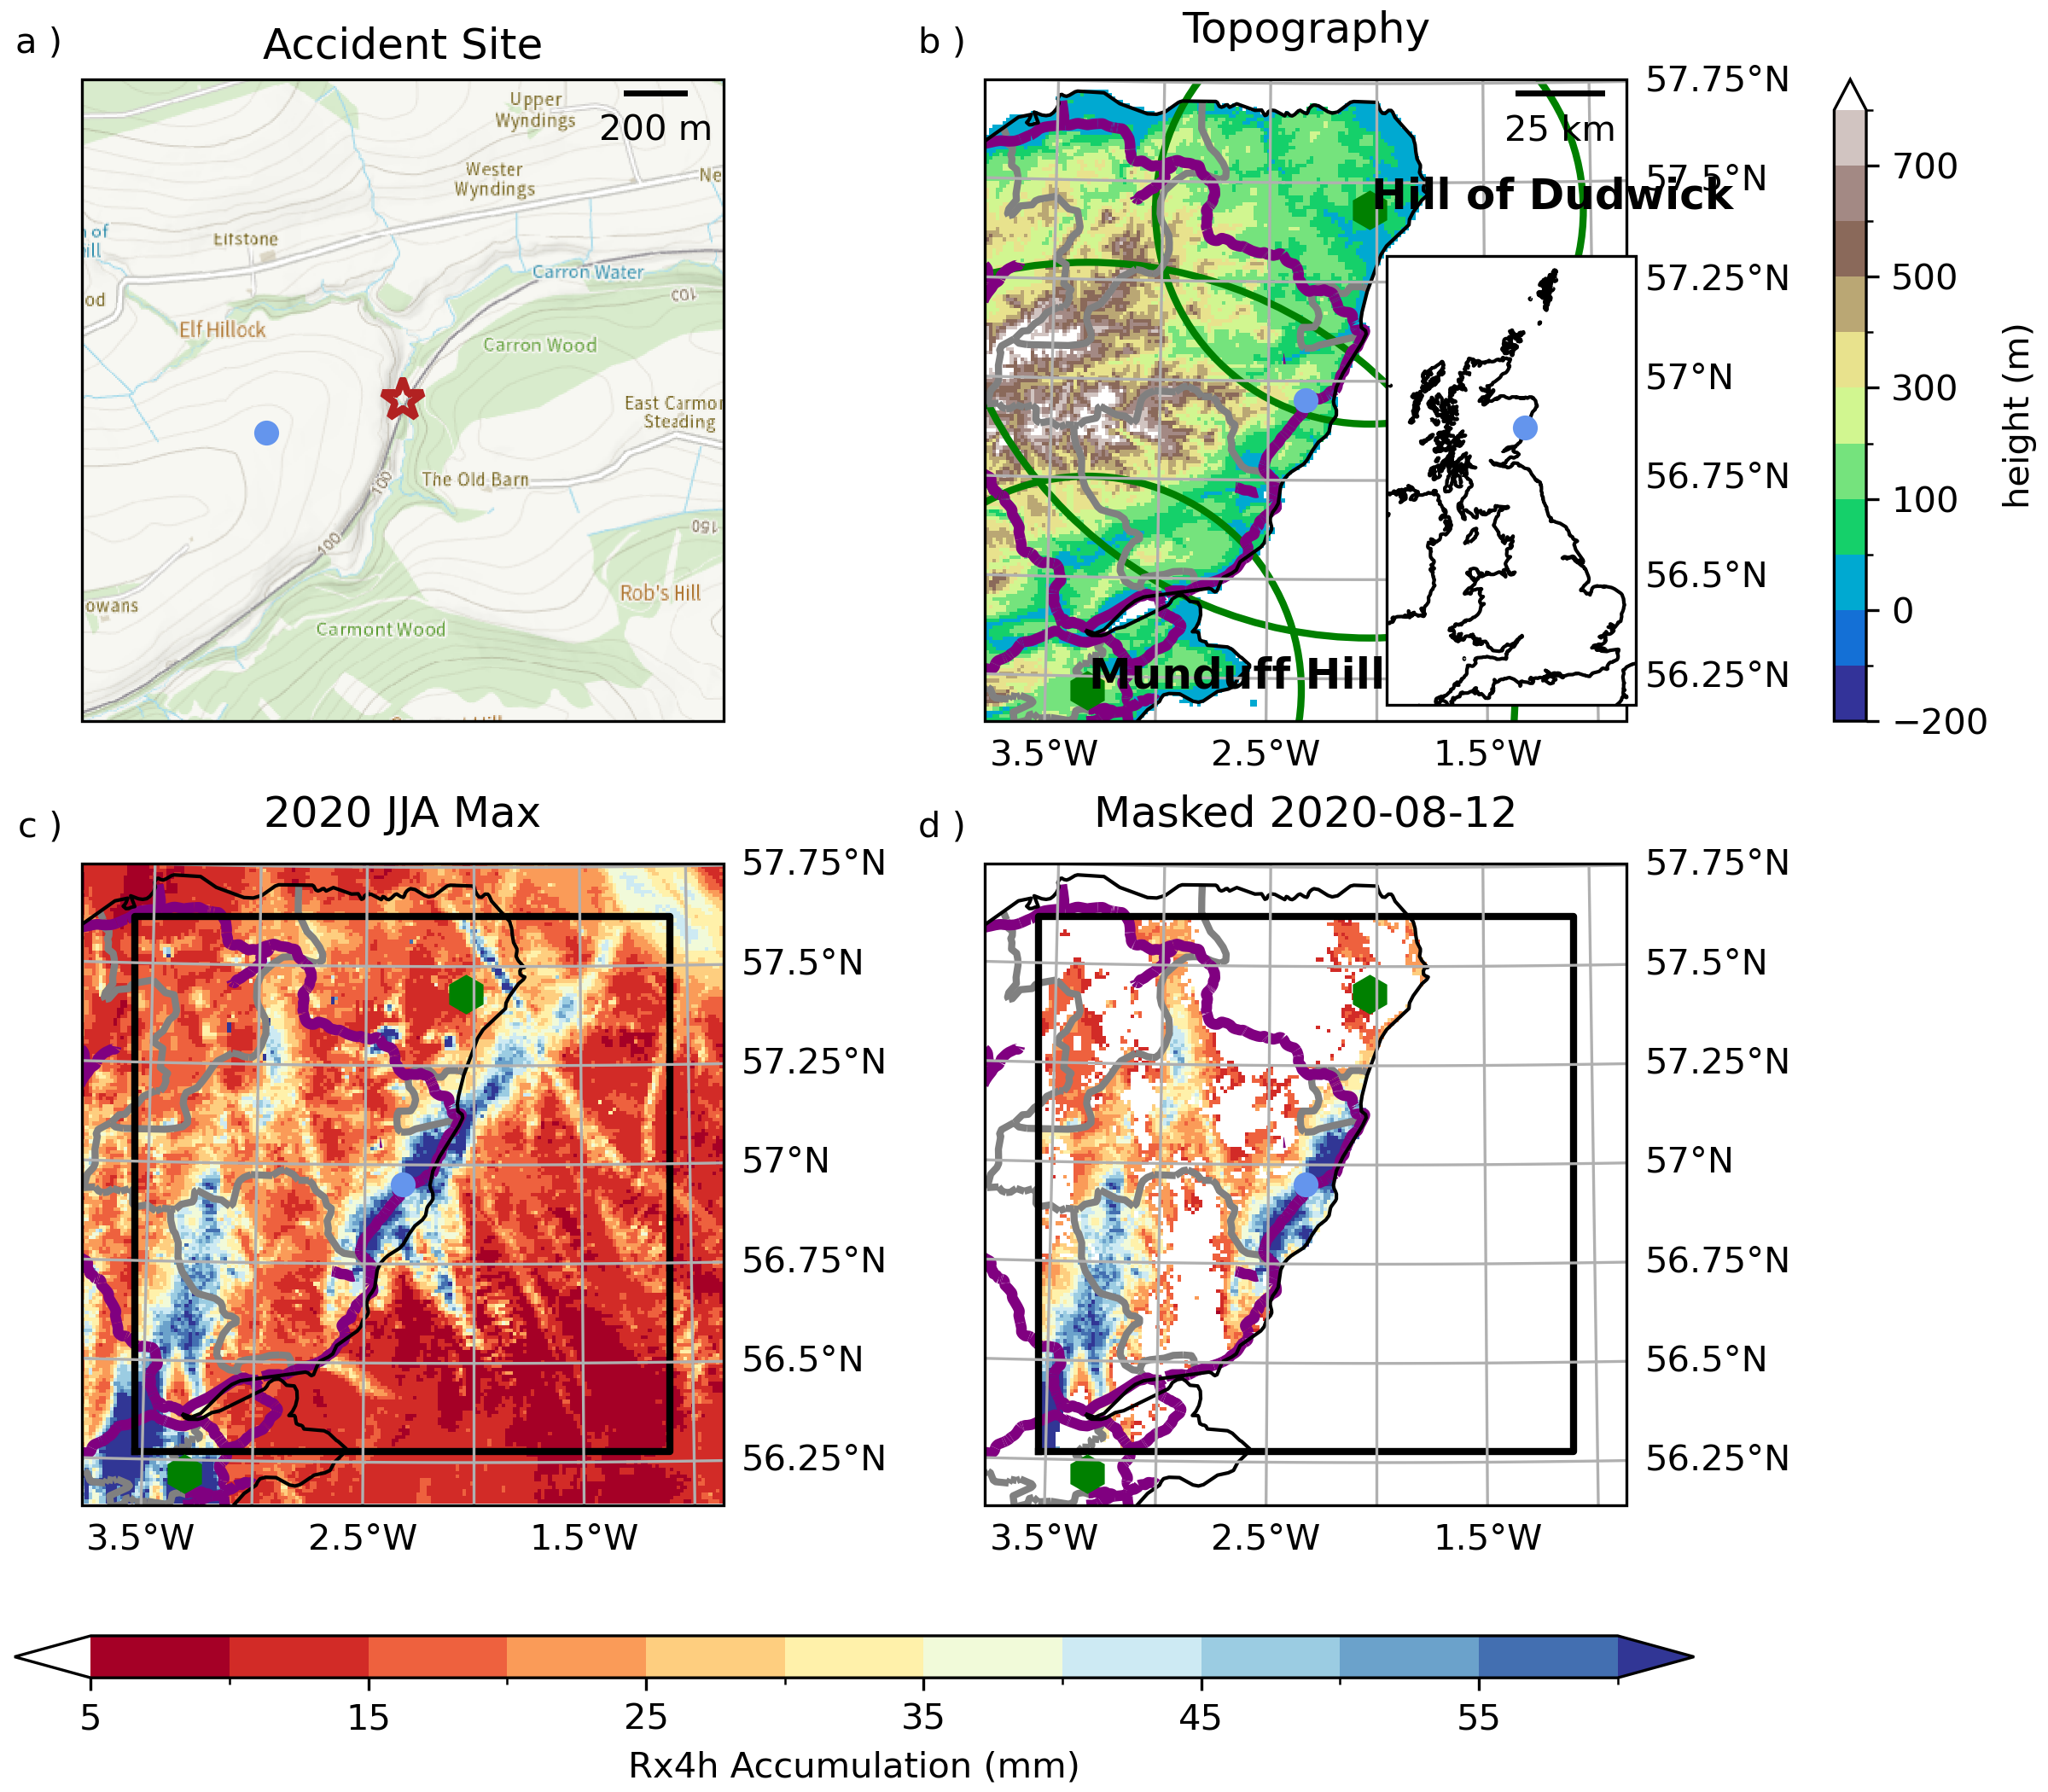
\includegraphics[width=\linewidth]{carmont_geog_group}
	\caption{a) Topography of North East Scotland (at 1km resolution). Also shown, by their first two letters, are the locations of Dyce, Aviemore, Aberdeen, Stonehaven and Montrose. Inset shows Great Britain and Ireland. Colour scale on bar to right. Circles are  60 and 120 km from radar stations (green hexagons with full names). b)  Map of Carmont accident site -- brick-red star shows where train derailed. Main features are contour lines every 10 meters, railway (black line) and woods (green) (Map crown copyright Ordinance Survey).  c) Maximum 4 hour radar rainfall accumulation (Rx4h)  for JJA 2020. d) Event of 2020-08-21 with coloured cells showing Rx4h that occur on 2020-08-21.  White are cells that do not form part of this event.  The black box in c \& d shows the 150x150 km region of interest. Scale bars are shown in a and b. Location of Carmont drain shown in all plots as pale blue dot.  }
	\label{fig:carmont_geog_group}
\end{figure}
\clearpage
\begin{figure}[ht!]
	\centering
	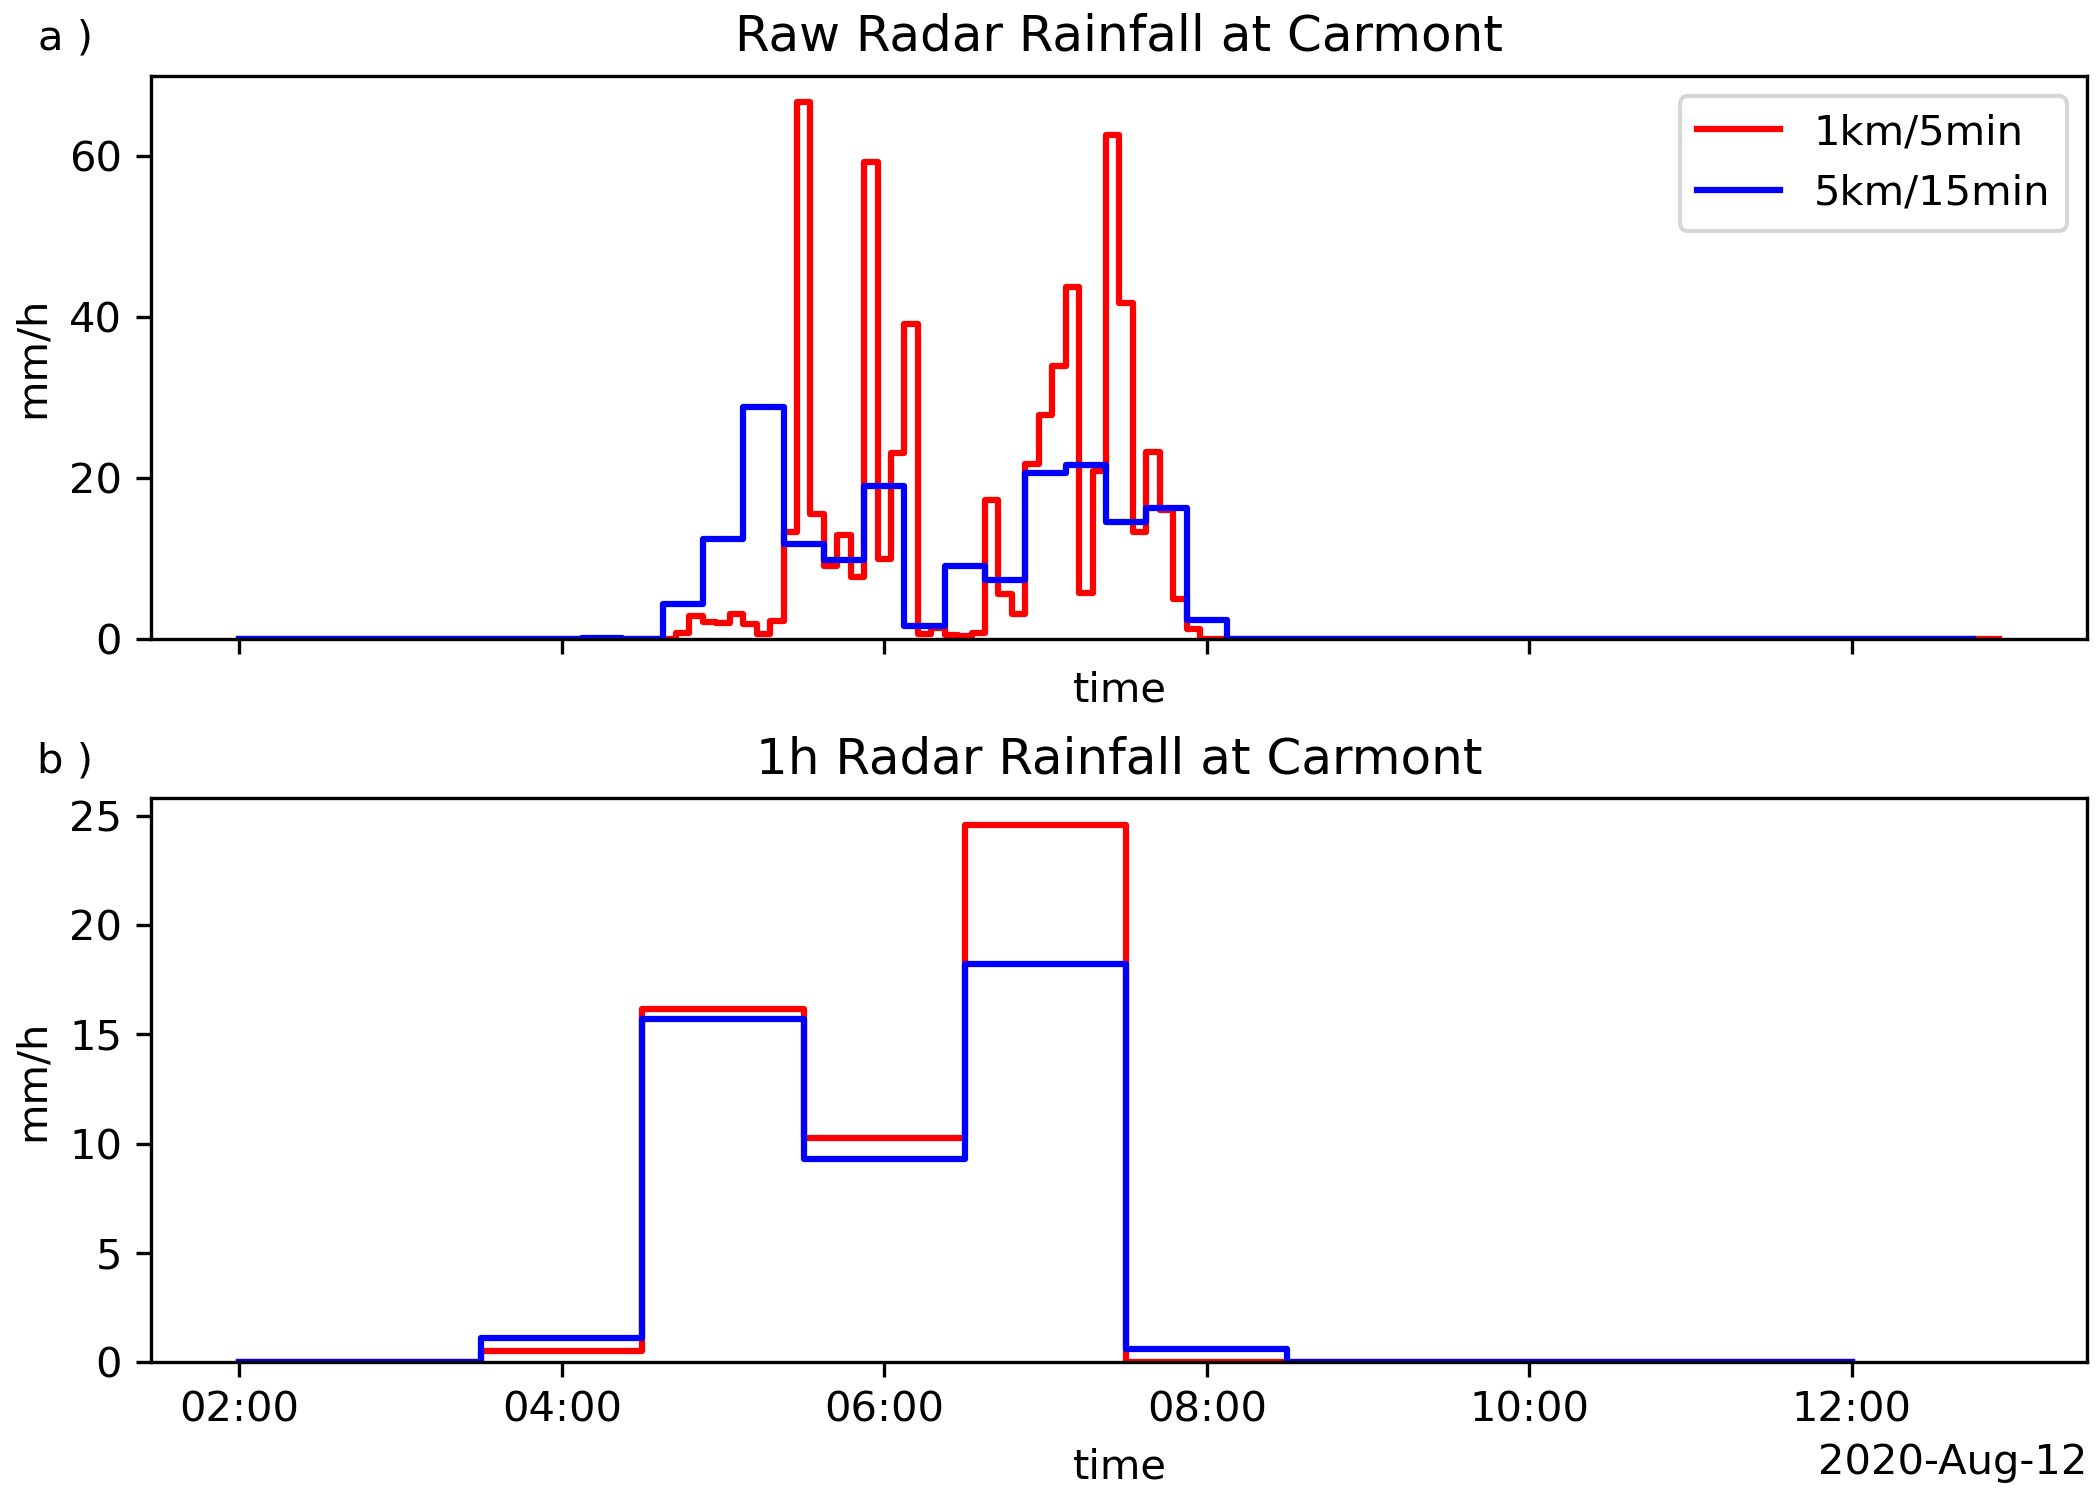
\includegraphics[width=0.5\linewidth]{radar_carmont}
	\caption{a) Radar rainfall rates at Carmont (mm/h) for 1km/5 min (red) and 5km/15 min. Dotted lines show accumulation reaching 51.5 and 44.9 mm for the 1km \& 5km data respectively. Circles show when 1/2 the total rain has fallen; b) Hourly mean rates for 1km (red) and 5km (blue) radar data. Data is shown from 2020-08-12T02:45 to 10:15 and ``Derail'' shows when the train derailed. }
	\label{fig:aug2020_rain}
\end{figure}

\begin{figure}[ht!]
	\centering
	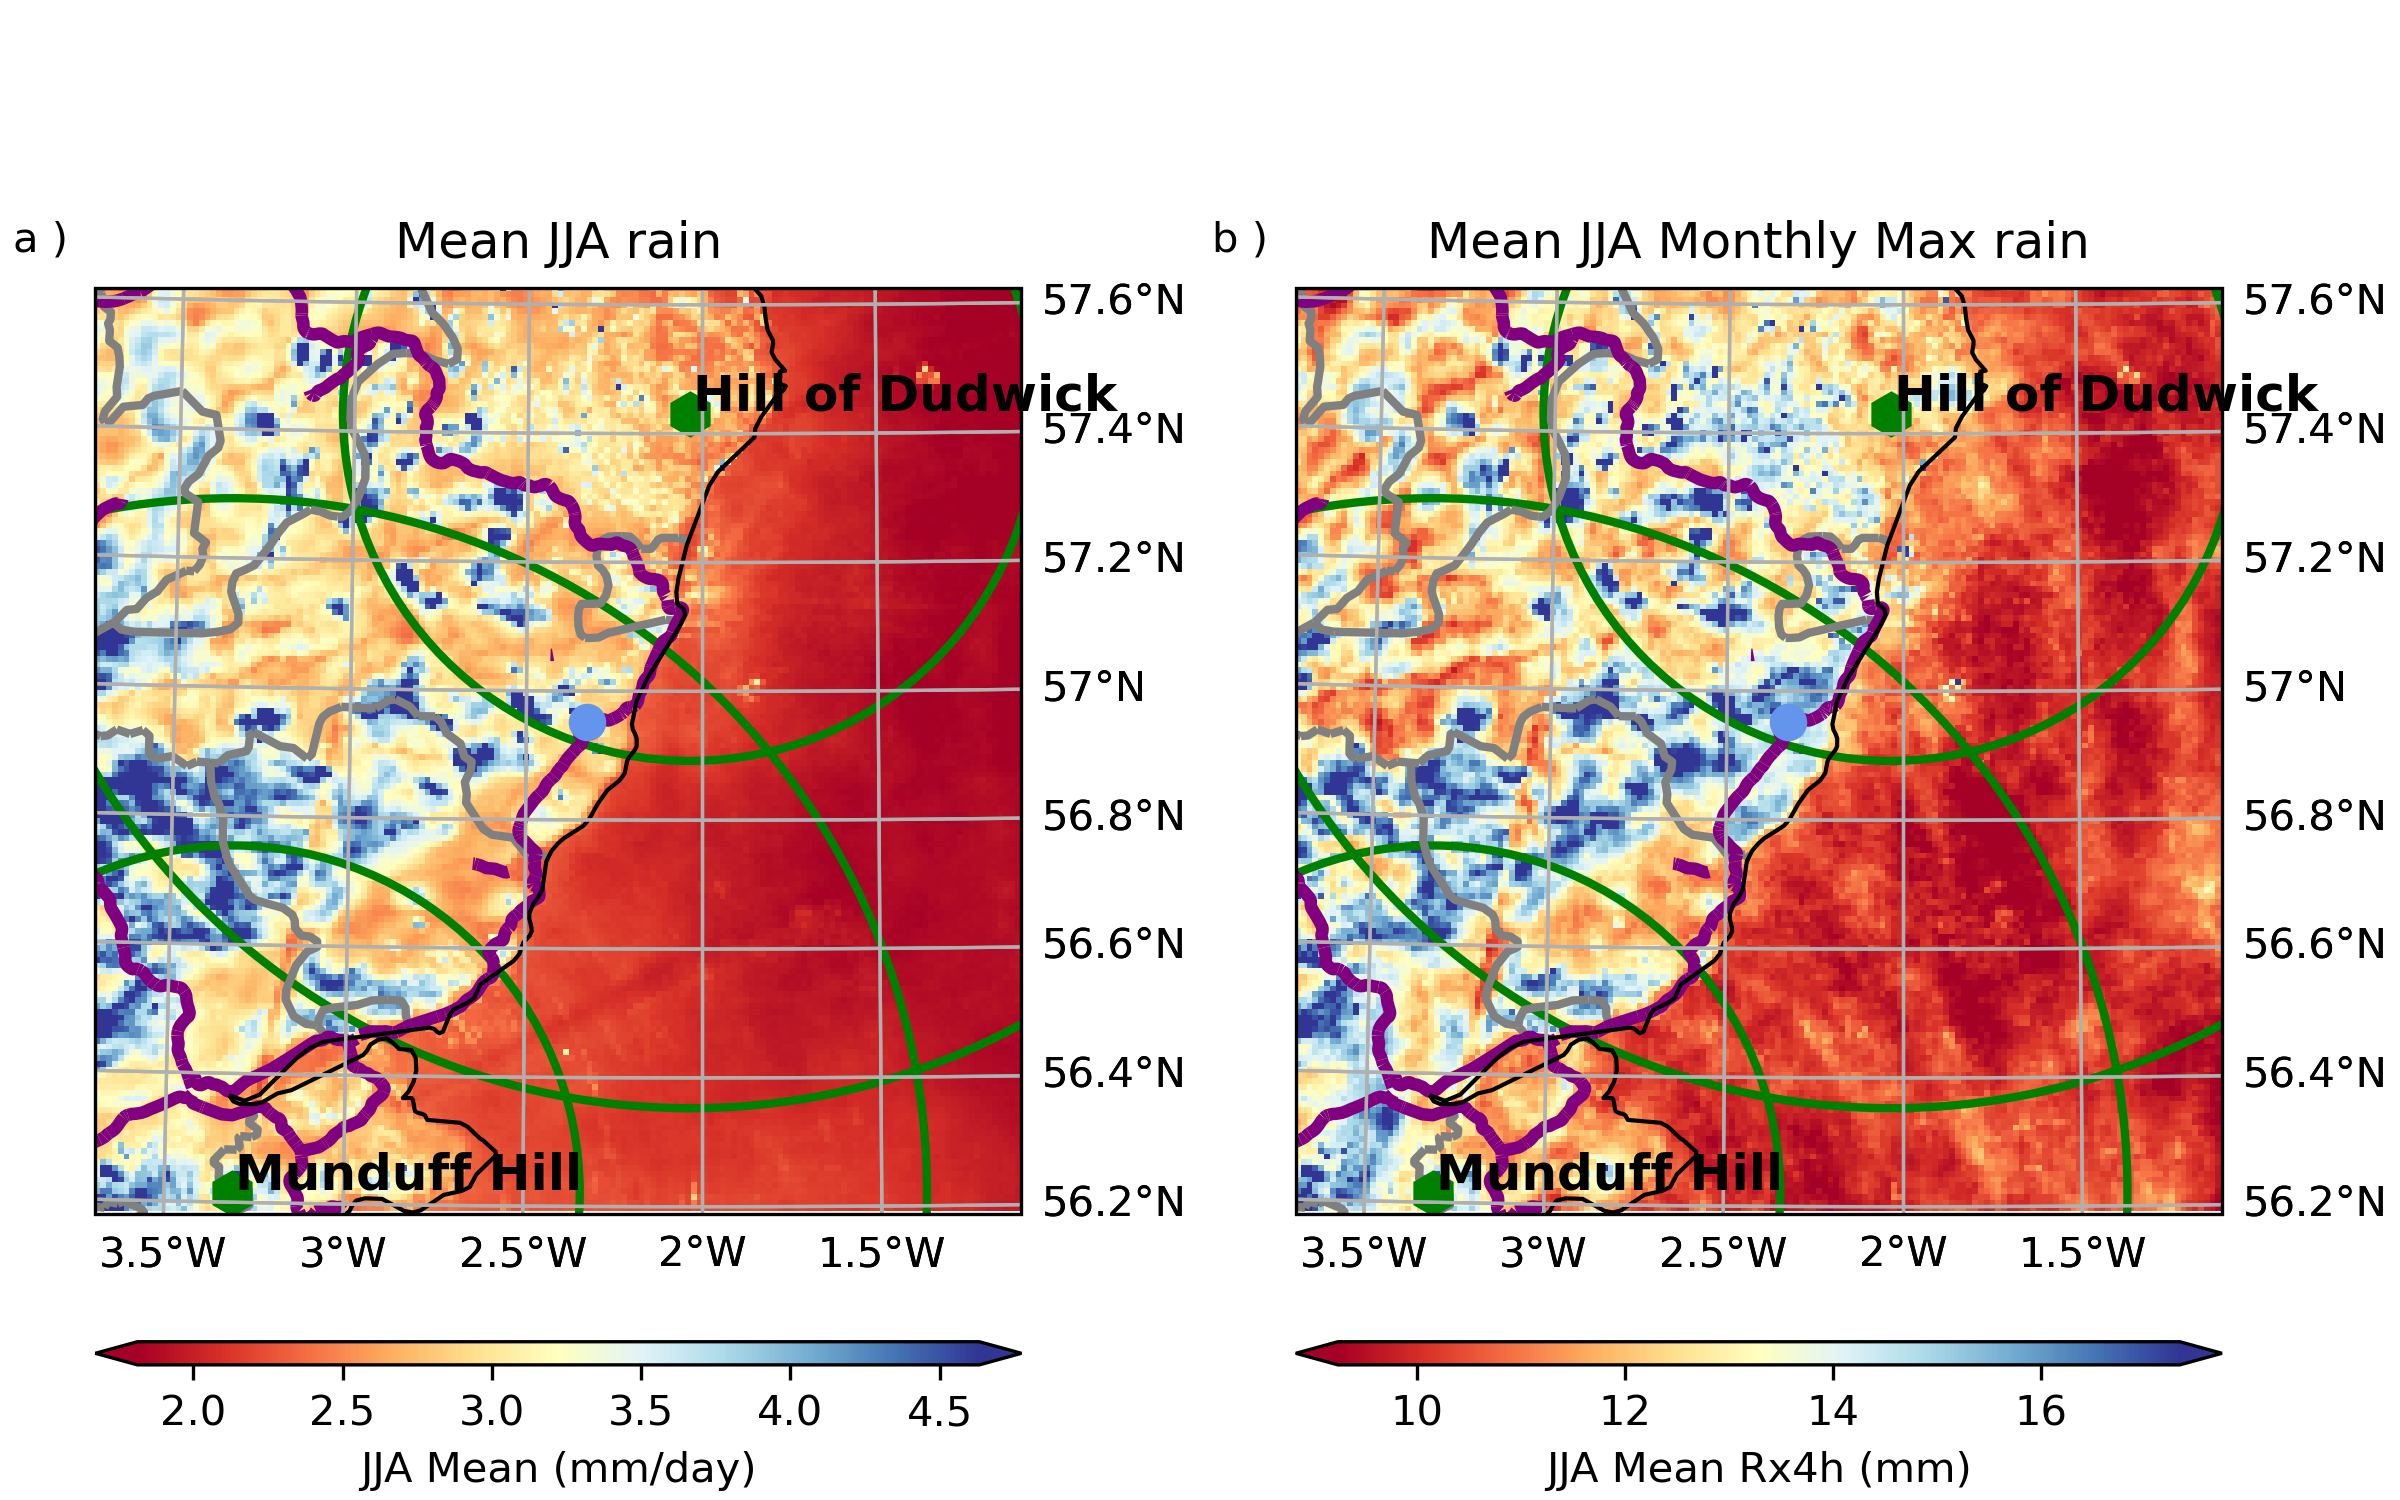
\includegraphics[width=\linewidth]{radar_jja}
	\caption{a) Mean radar rainfall (mm/day) b) Median monthly Rx4h(mm). Values are for summers (June-July-August) from 2008 to 2023 inclusive. Circles are  60 and 120 km from radar stations (Green hexagons). The pale blue circle shows the point ("Carmont drain") where rain occurred, purple lines show railways and grey lines local authority boundaries. Semi-transparent green lines (circles) show radial features (localised sources) which may be radar artefacts. }
	\label{fig:radar_jja}
\end{figure}


\begin{figure}
	\centering
	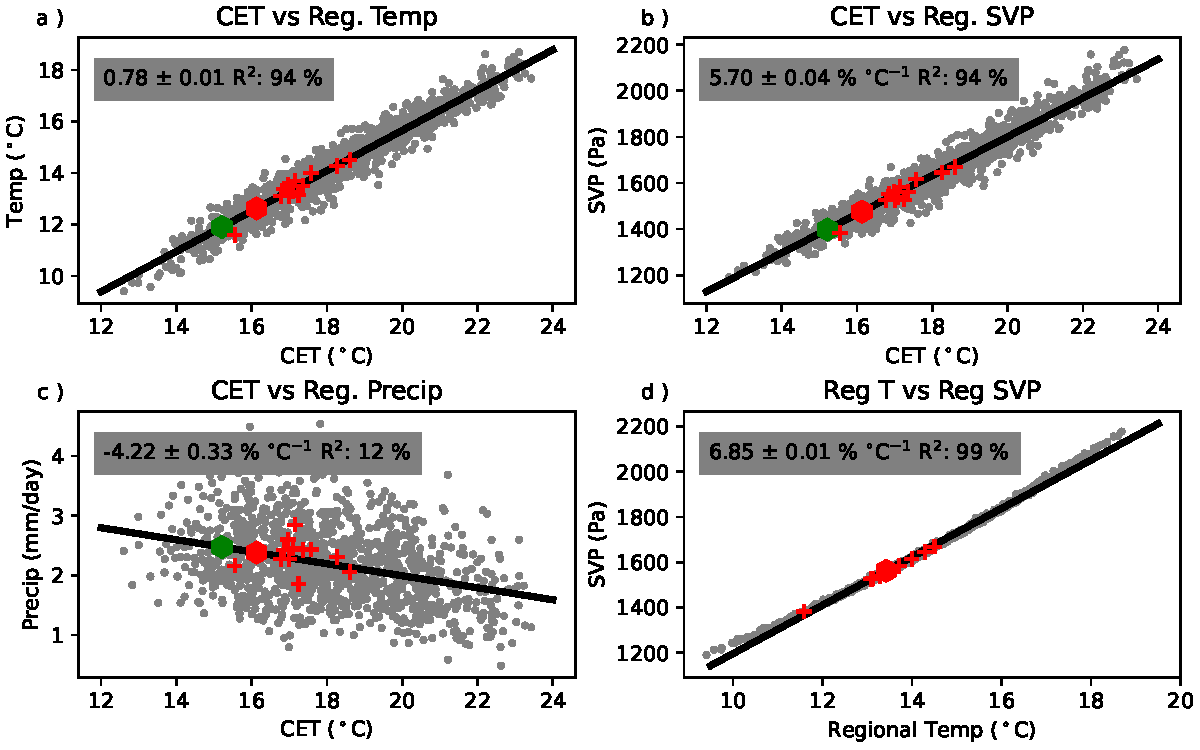
\includegraphics[width=\linewidth]{scatter}
	\caption{Scatter plots for CPM simulated summer mean  a)  Central England Temperature (CET) vs  regional mean temperature; b) CET vs regional average saturated vapour pressure (SVP); c) CET vs regional average precipitation; d) Regional temperature vs Regional SVP. In plots a-c, green, red and blue hexagons show  estimated 1850-1899, 2008-2023 \& $+2^\circ$C average values  using regression predictions from observed, and 1850-1899 average $+1.84^\circ$ CET values respectively. Lines show linear best fits. Red crosses show, for each ensemble member, mean simulated values for 2008-2023. Text shows  change, and standard error, for  $1^{\circ}$C change in CET or Regional Temperature, and $R^2$ of fit.}
	\label{fig:cet_scatter}
\end{figure}

\begin{figure}
	\centering
	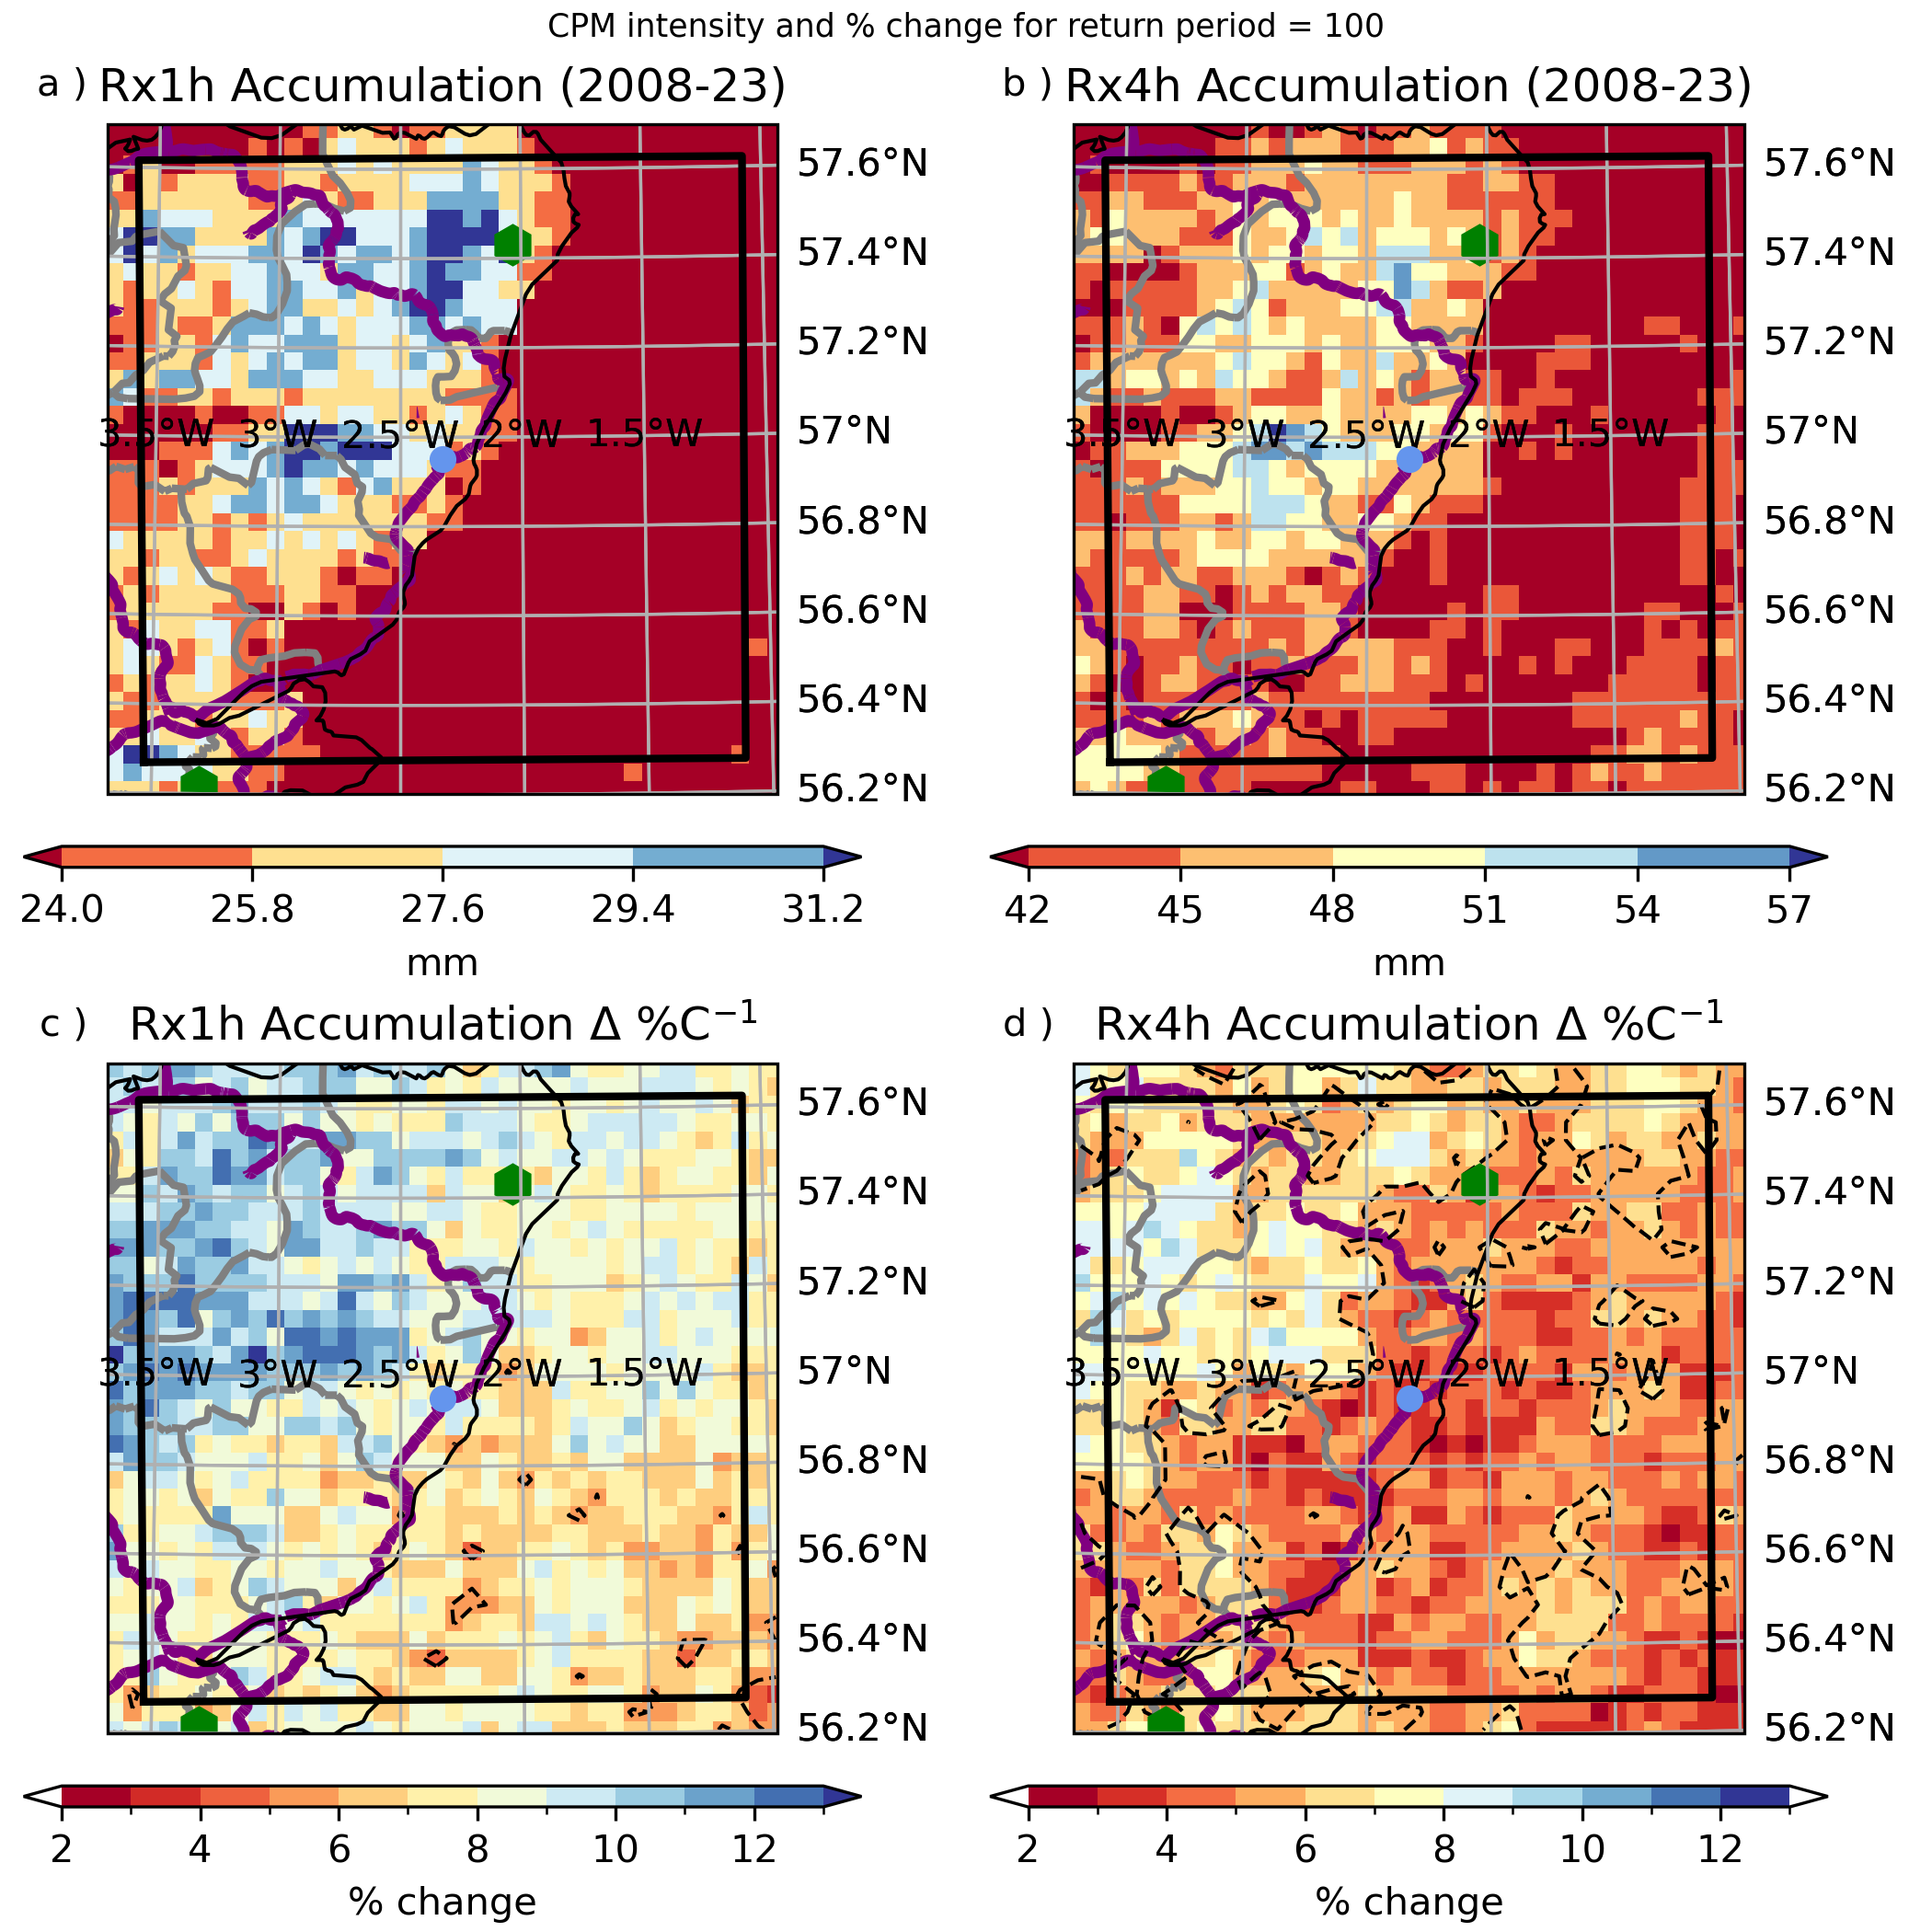
\includegraphics[width=1\linewidth]{cpm_intensity_delta}
	\caption{One in a hundred-summer CPM Rx1h(a) \& Rx4h(c) and percentage sensitivity to 1 degree CET increase for Rx1h(b) and Rx4h(d).  a \& c colour table levels are $\pm$ 15\% of the values at Carmont Drain. Dashed lines (b \& d) shows intensity increase of 5.7\%/degree CET, corresponding to CC. Other elements as Figure~\ref{fig:radar_jja}.  }
	\label{fig:map_intensity}
\end{figure}

\begin{figure}
	\centering
	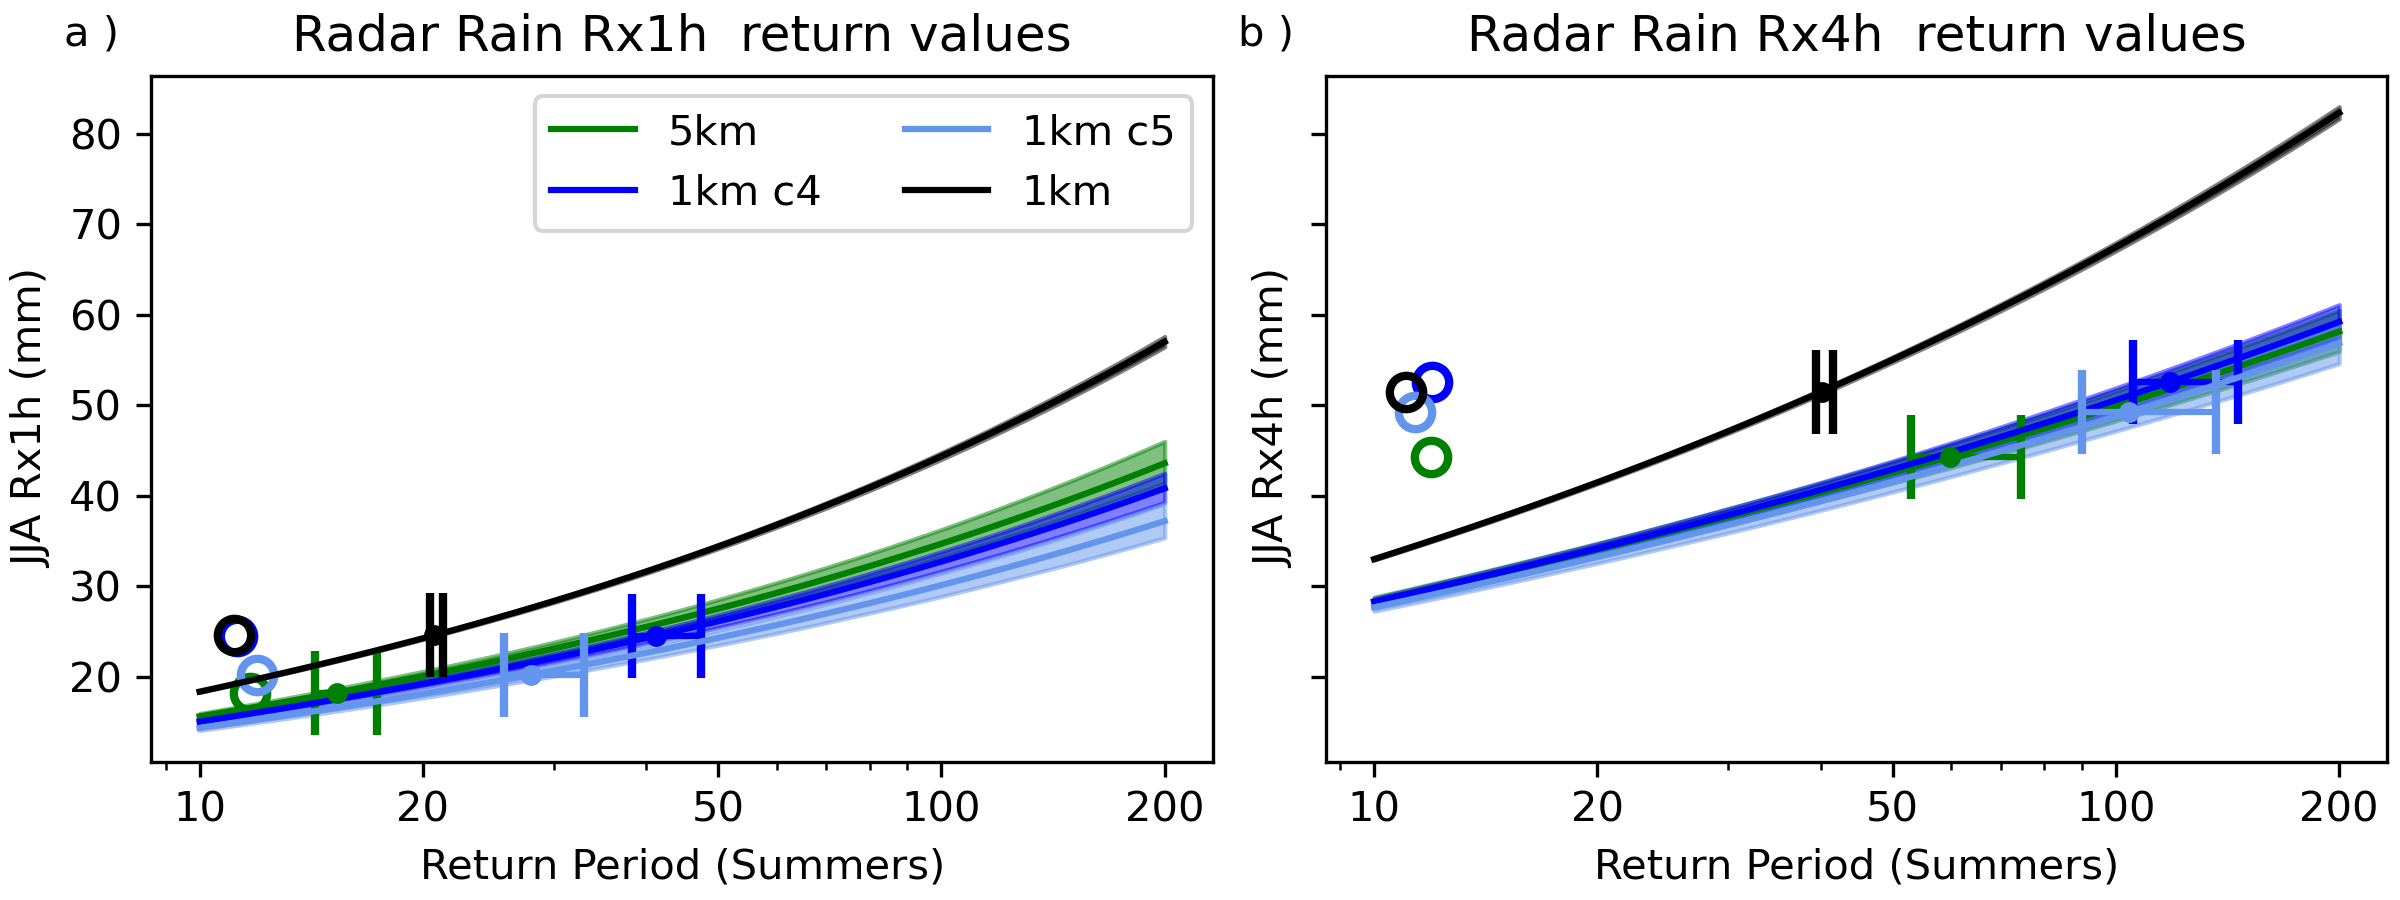
\includegraphics[width=\linewidth]{radar_return_prds}
	\caption{Estimated return values for  JJA maximum accumulated radar rainfall. Shown are Rx1h (a) and Rx4h (b) for 1km  (black),  5km (green), 1km-c4 (blue) and 1km-c5 (pale blue) radar rain. Symbols in left hand of sub-plots show radar rain at nearest grid point to Carmont drain. Horizontal error bars show 5-95\% return period uncertainty ranges. }
	\label{fig:radar_rtn_prd}
\end{figure}

\begin{figure}
	\centering
	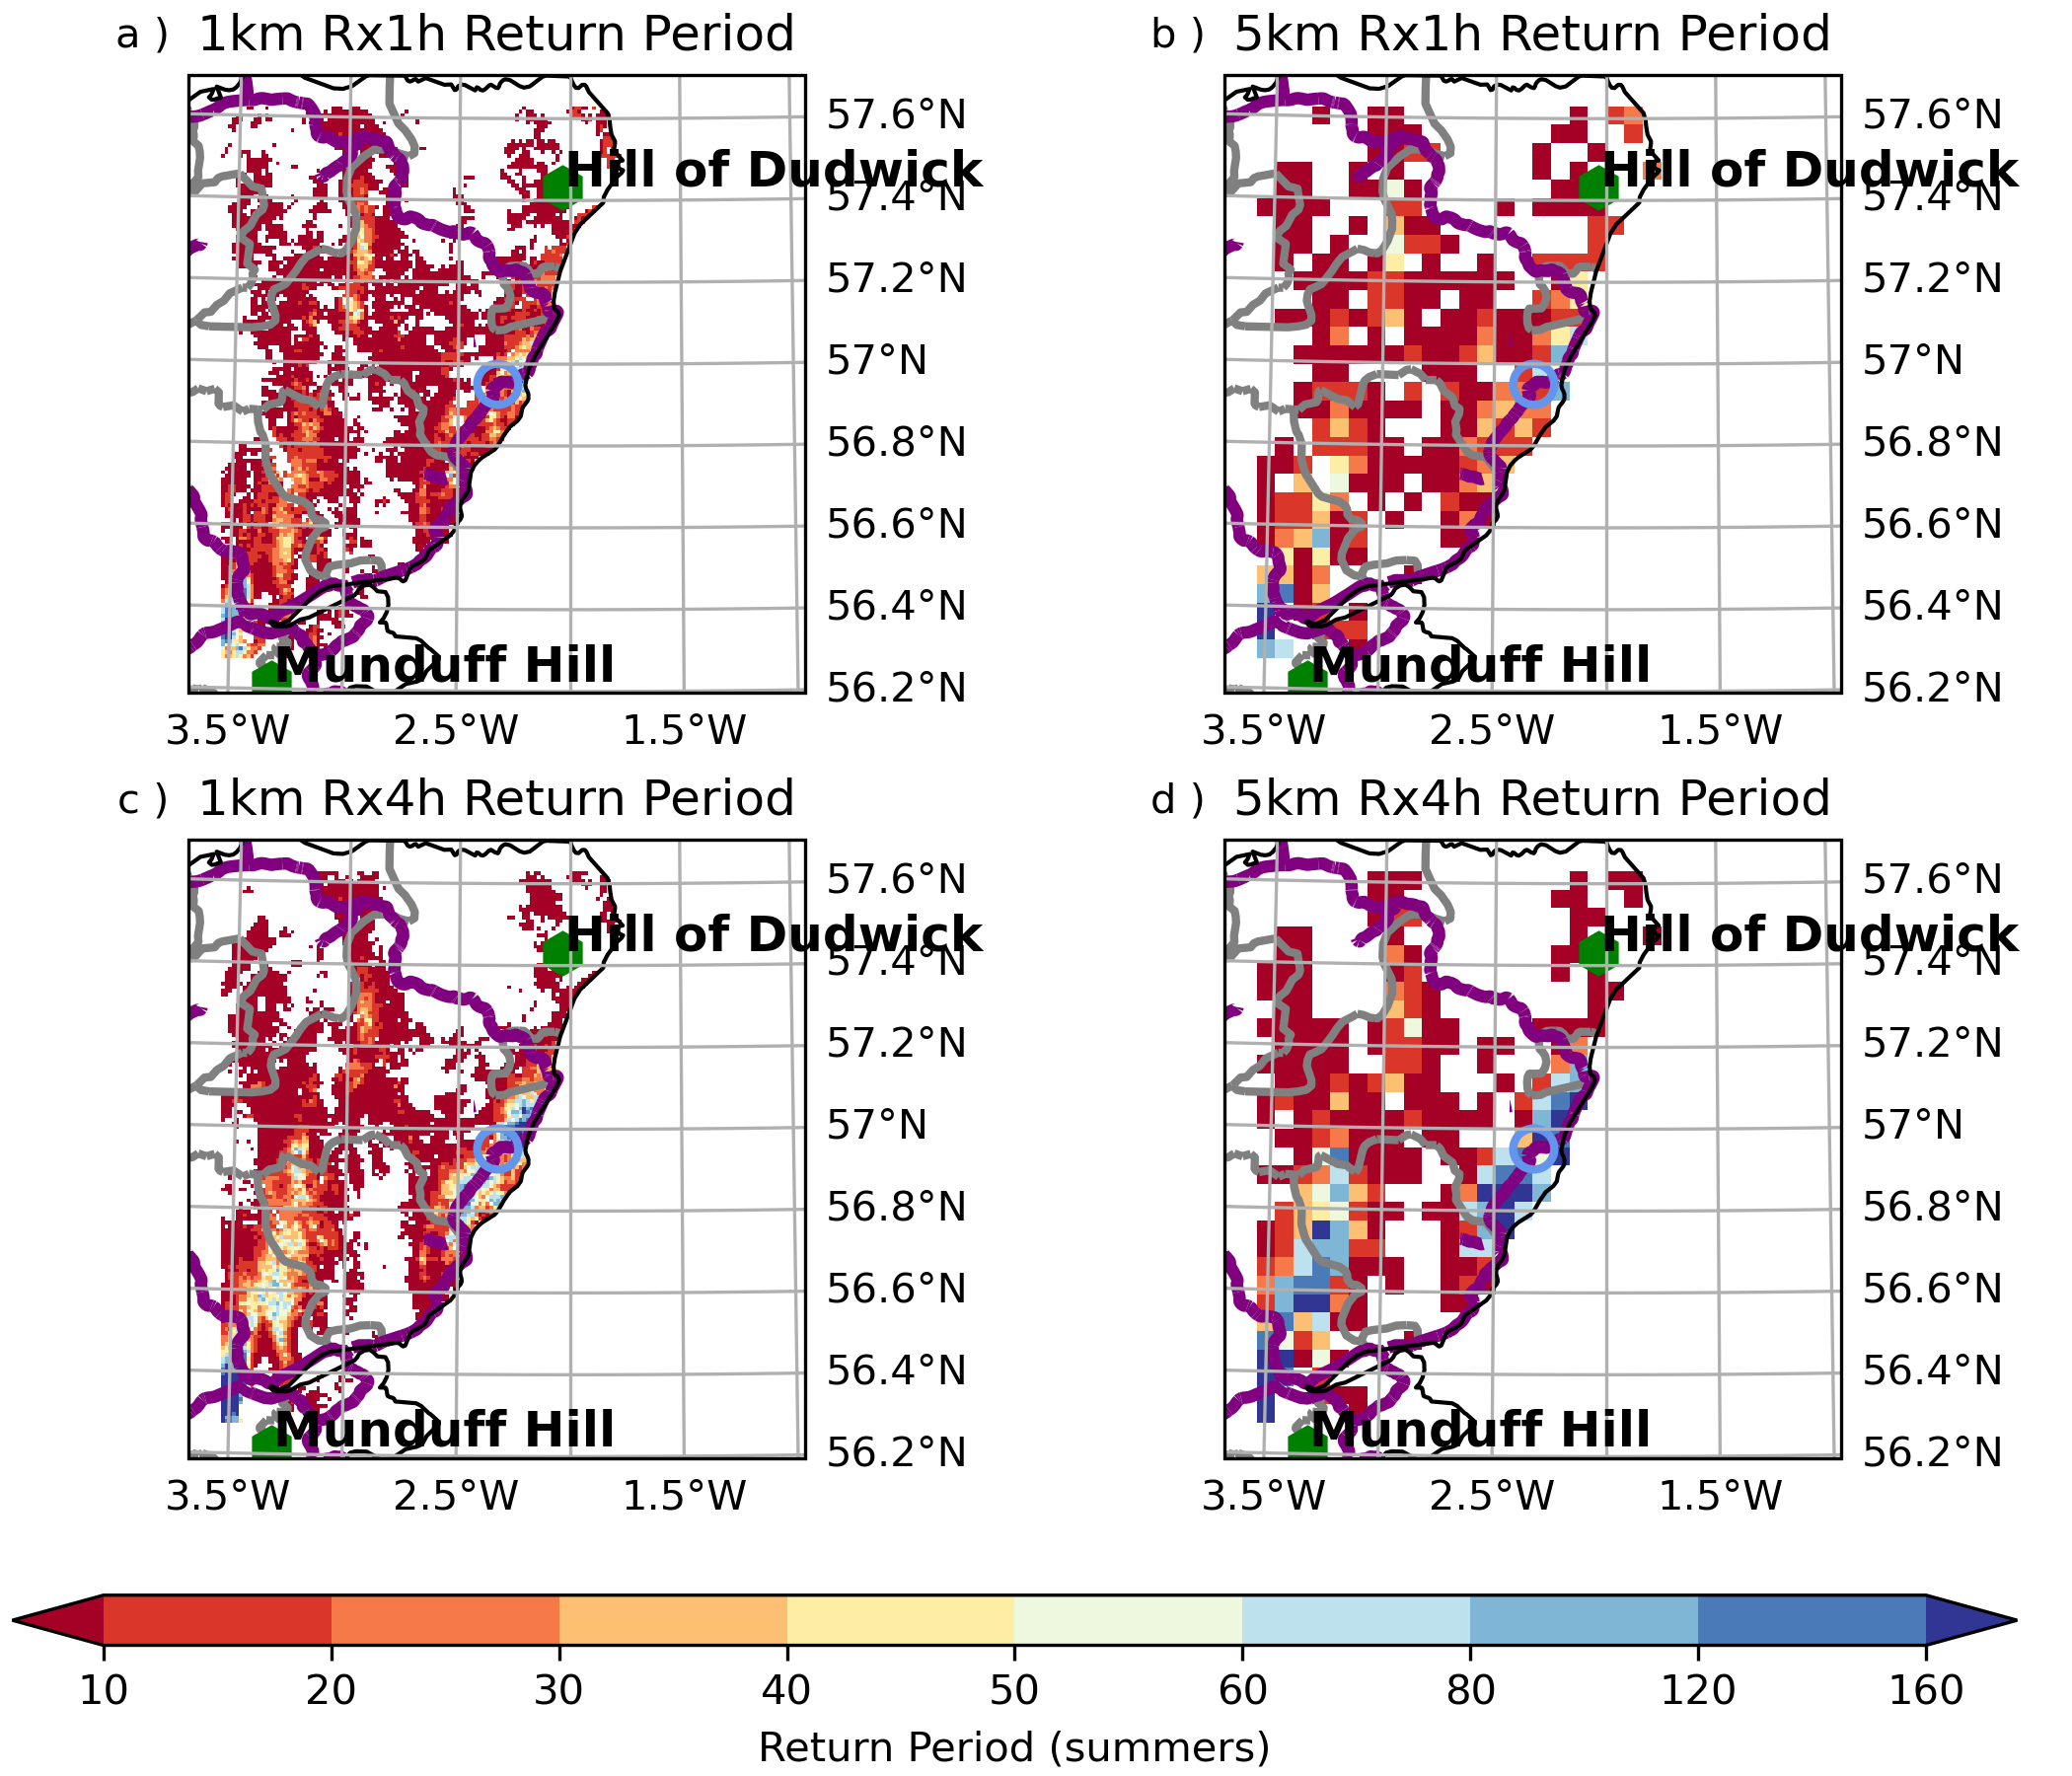
\includegraphics[width=\linewidth]{map_return_prds}
	\caption{Return periods for Carmont regional Rx1h (a \& b) and Rx4h (c \& d), which occurred on 2020-08-12. Plots a \& c show 1km data while plots c \& d show 5km data. The colour bar at the bottom refers to all plots. Other elements as Figure~\ref{fig:radar_jja}. } 
	\label{fig:map_rtn_prd}
\end{figure}


\begin{figure}
	\centering
	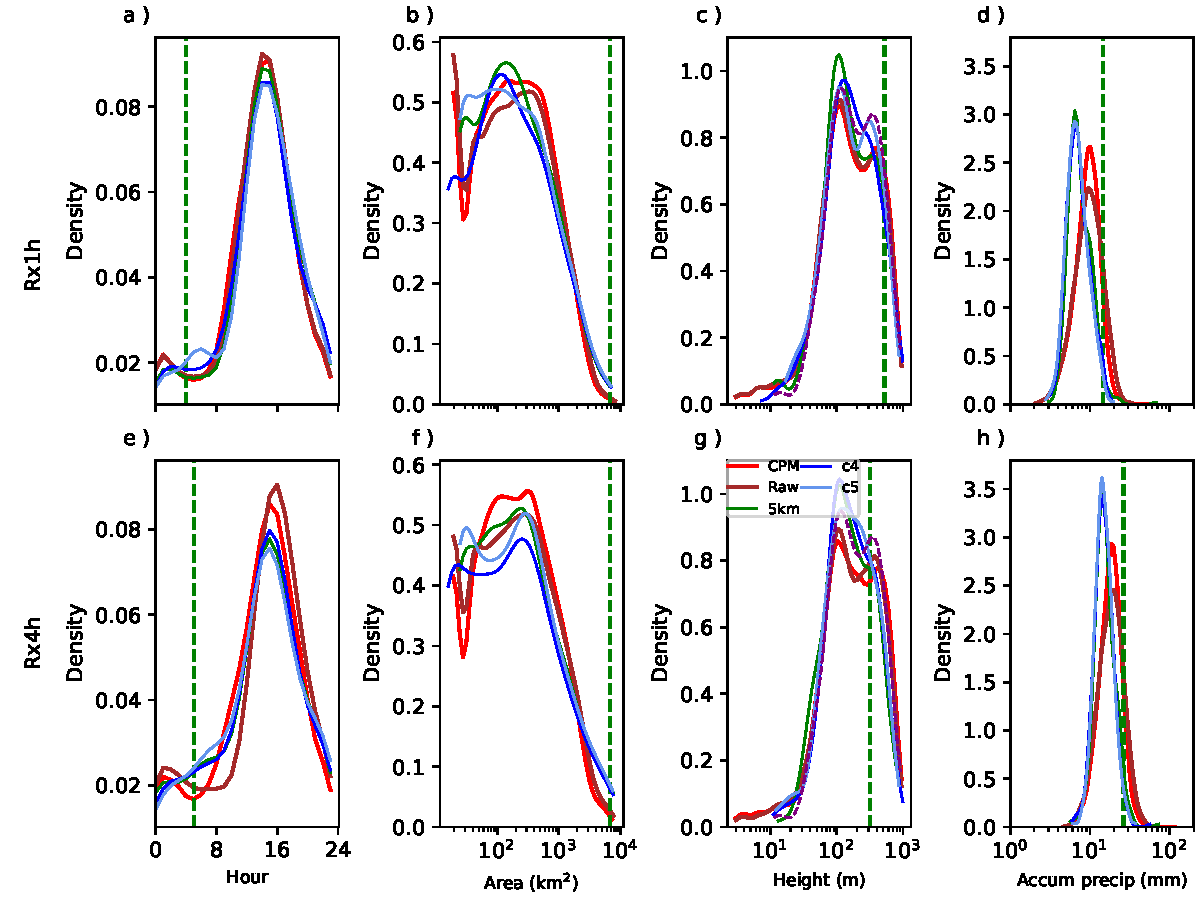
\includegraphics[width=\linewidth]{kde_smooth_events}
	\caption{Kernel Density Estimates (KDE) from  CPM (orange), CPM-Raw (brown), 5km radar (green), 1km-c4 (blue) and 1km-c5 (pale blue) events at 50\% quantile for 2008-2023 period.
		 Shown are day-hour (a \& e), event area (b \& f),  topographic height (c \& g ) and maximum Rainfall accumulation (d \& h). All plots, except a \& e, use a log x-axis. 
		  Top row shows Rx1h while bottom row shows Rx4h values. Shown in c \& g is the KDE for the 5km DEM topography. Vertical green lines shows values of 2020-08-12 for 5km radar dataset.}
	\label{fig:kde_smooth_events}
\end{figure}

\clearpage
\begin{figure}[ht!]
	\centering
	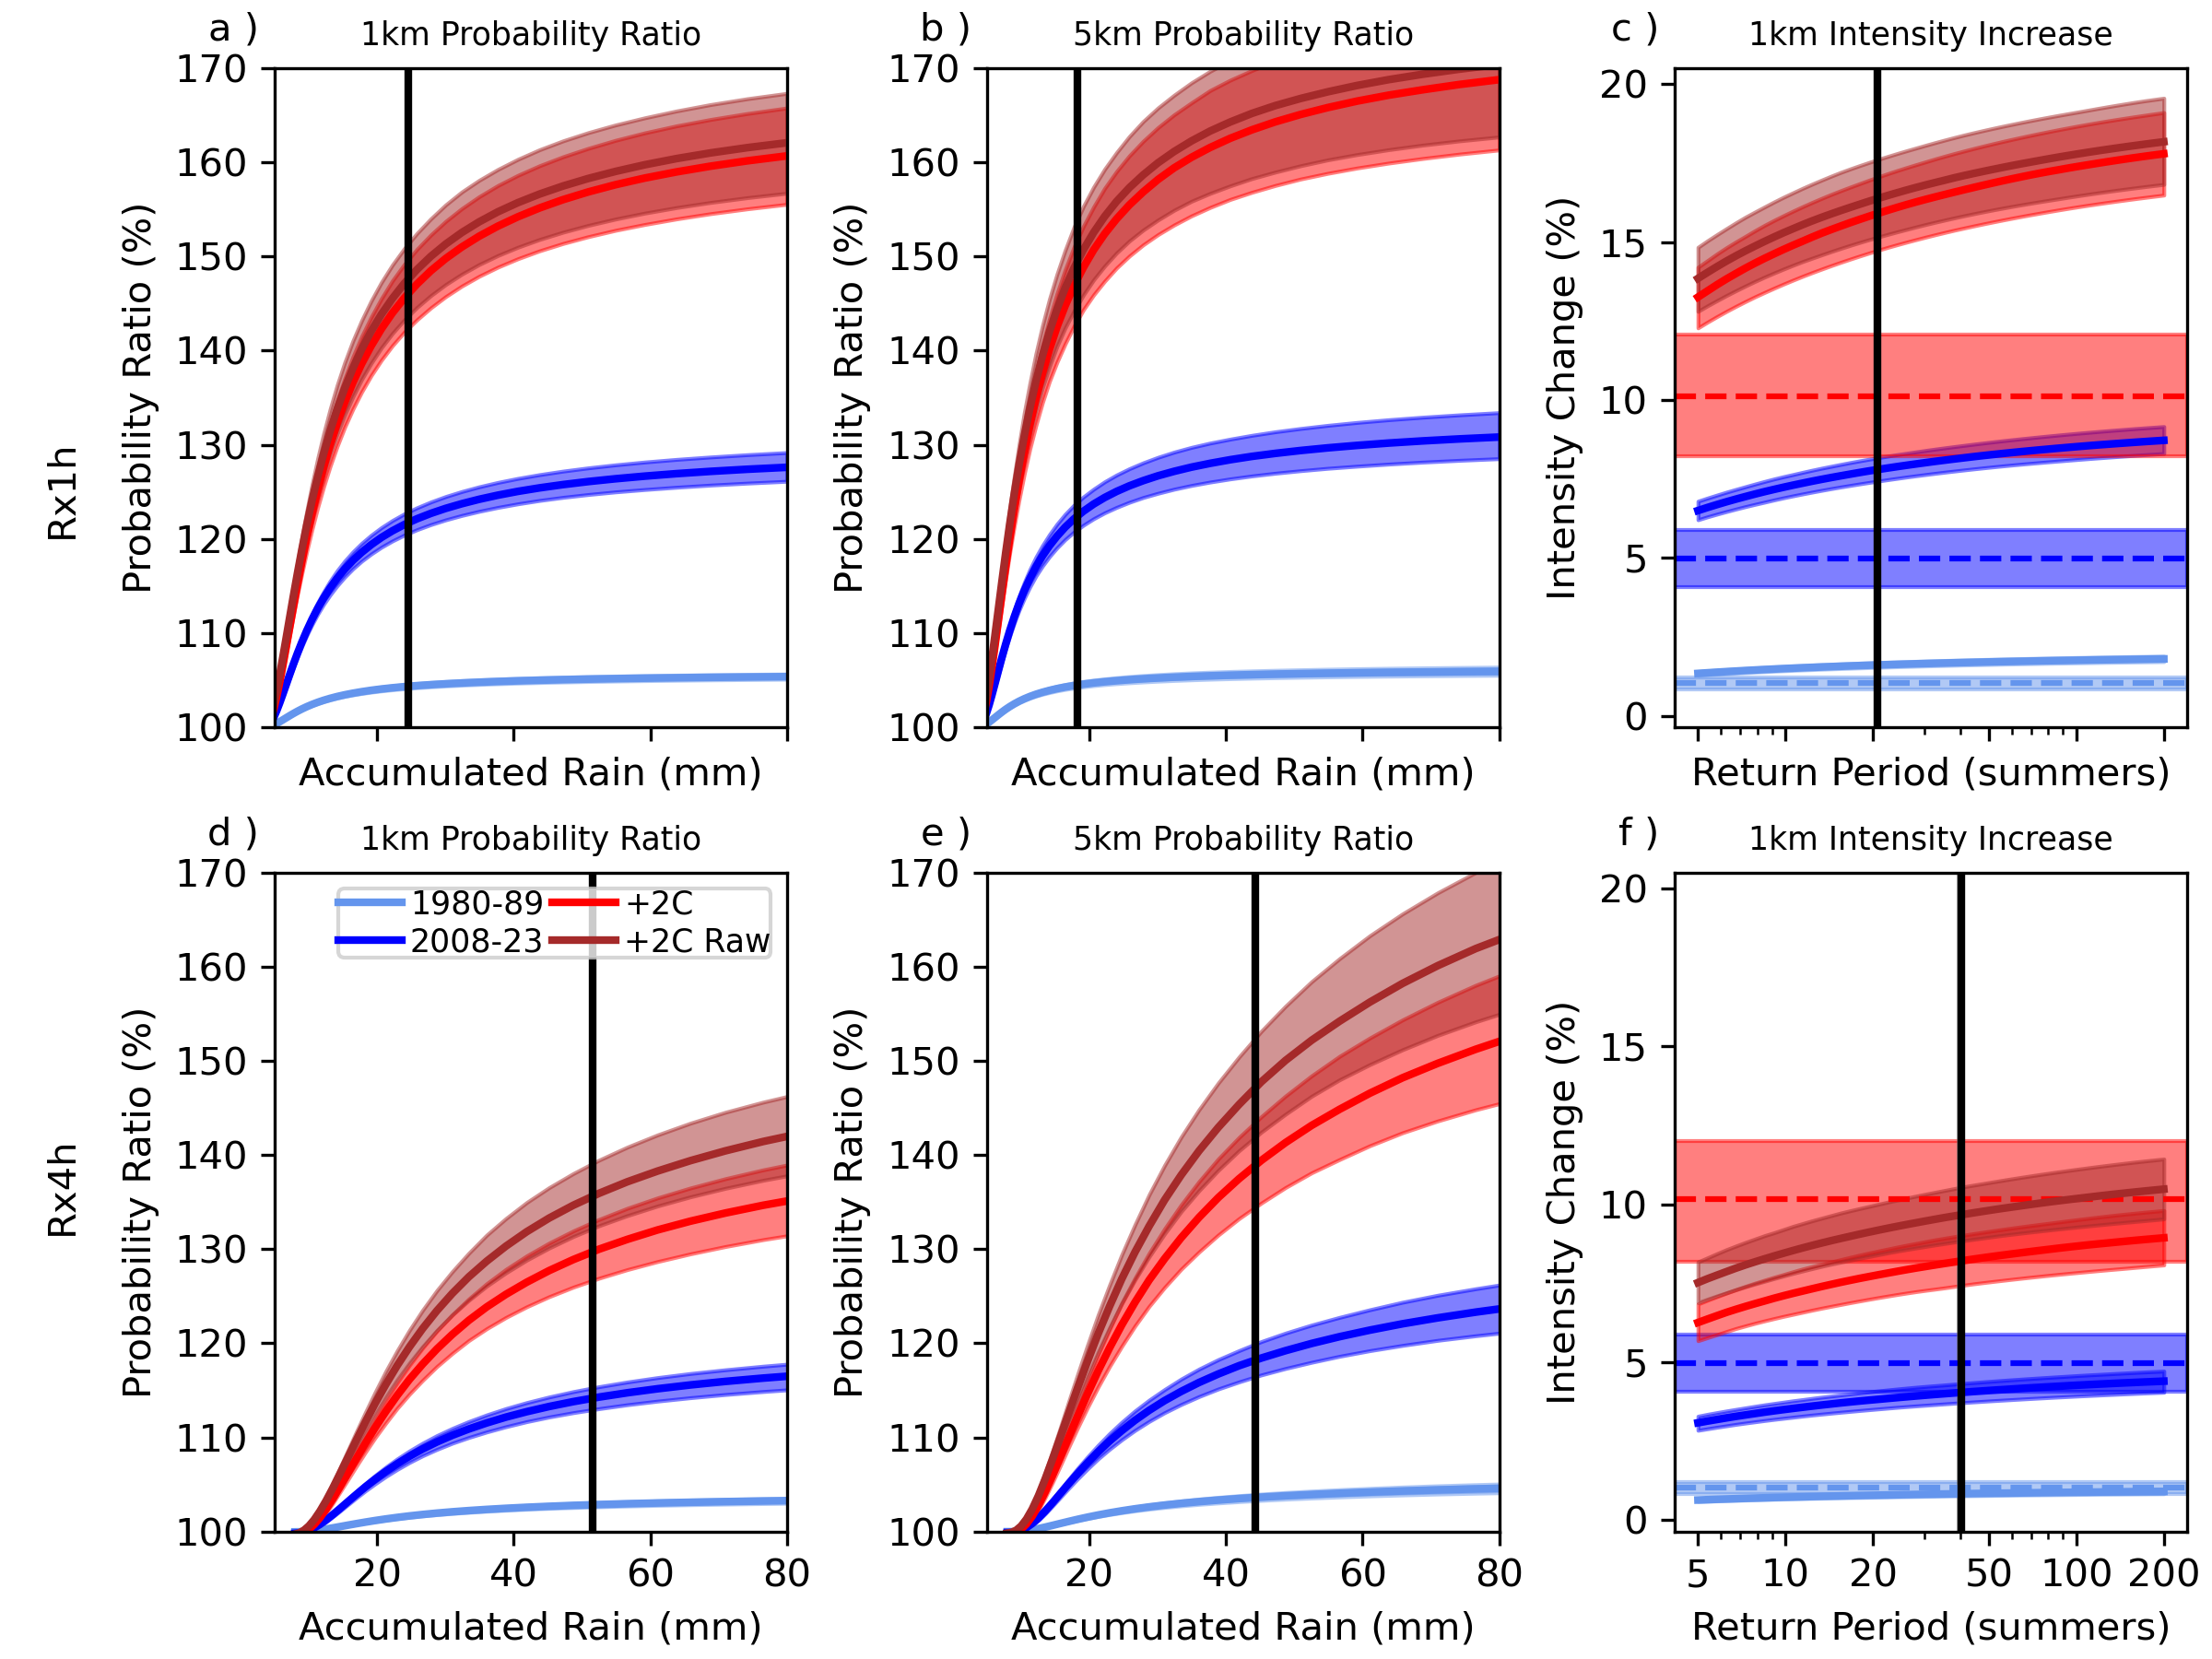
\includegraphics[width=0.9\linewidth]{intens_prob_ratios}
	\caption{a \& d: Probability ratio, relative to Pre-industrial, at Carmont drain as function of accumulated rainfall for 1km radar rainfall. b \& e) As a) but for 5km radar rainfall. c \& f: Intensity ratio at Carmont drain  as function of  return period. Also shown are median (horizontal dashed line) and 5-95\% uncertainties (vertical shading) for changes expected from Clausius-Clapeyron. Vertical black lines show computed return period for radar rain at Carmont. Upper plots (a-c) show Rx1h  while lower plots (d-f) show Rx4h accumulations. All plots show changes for +2C (red), 2012-2023 (dark blue) and 1980-1989 (pale blue) from filtered CPM data. Brown shows changes at +2C  when raw CPM data is used.   In all plots solid lines are median changes with 5-95\% uncertainty range shown by  shading.}
	\label{fig:intense_prob_ratios}
\end{figure}
\clearpage

%\begin{figure}[ht!]
%	\centering
%	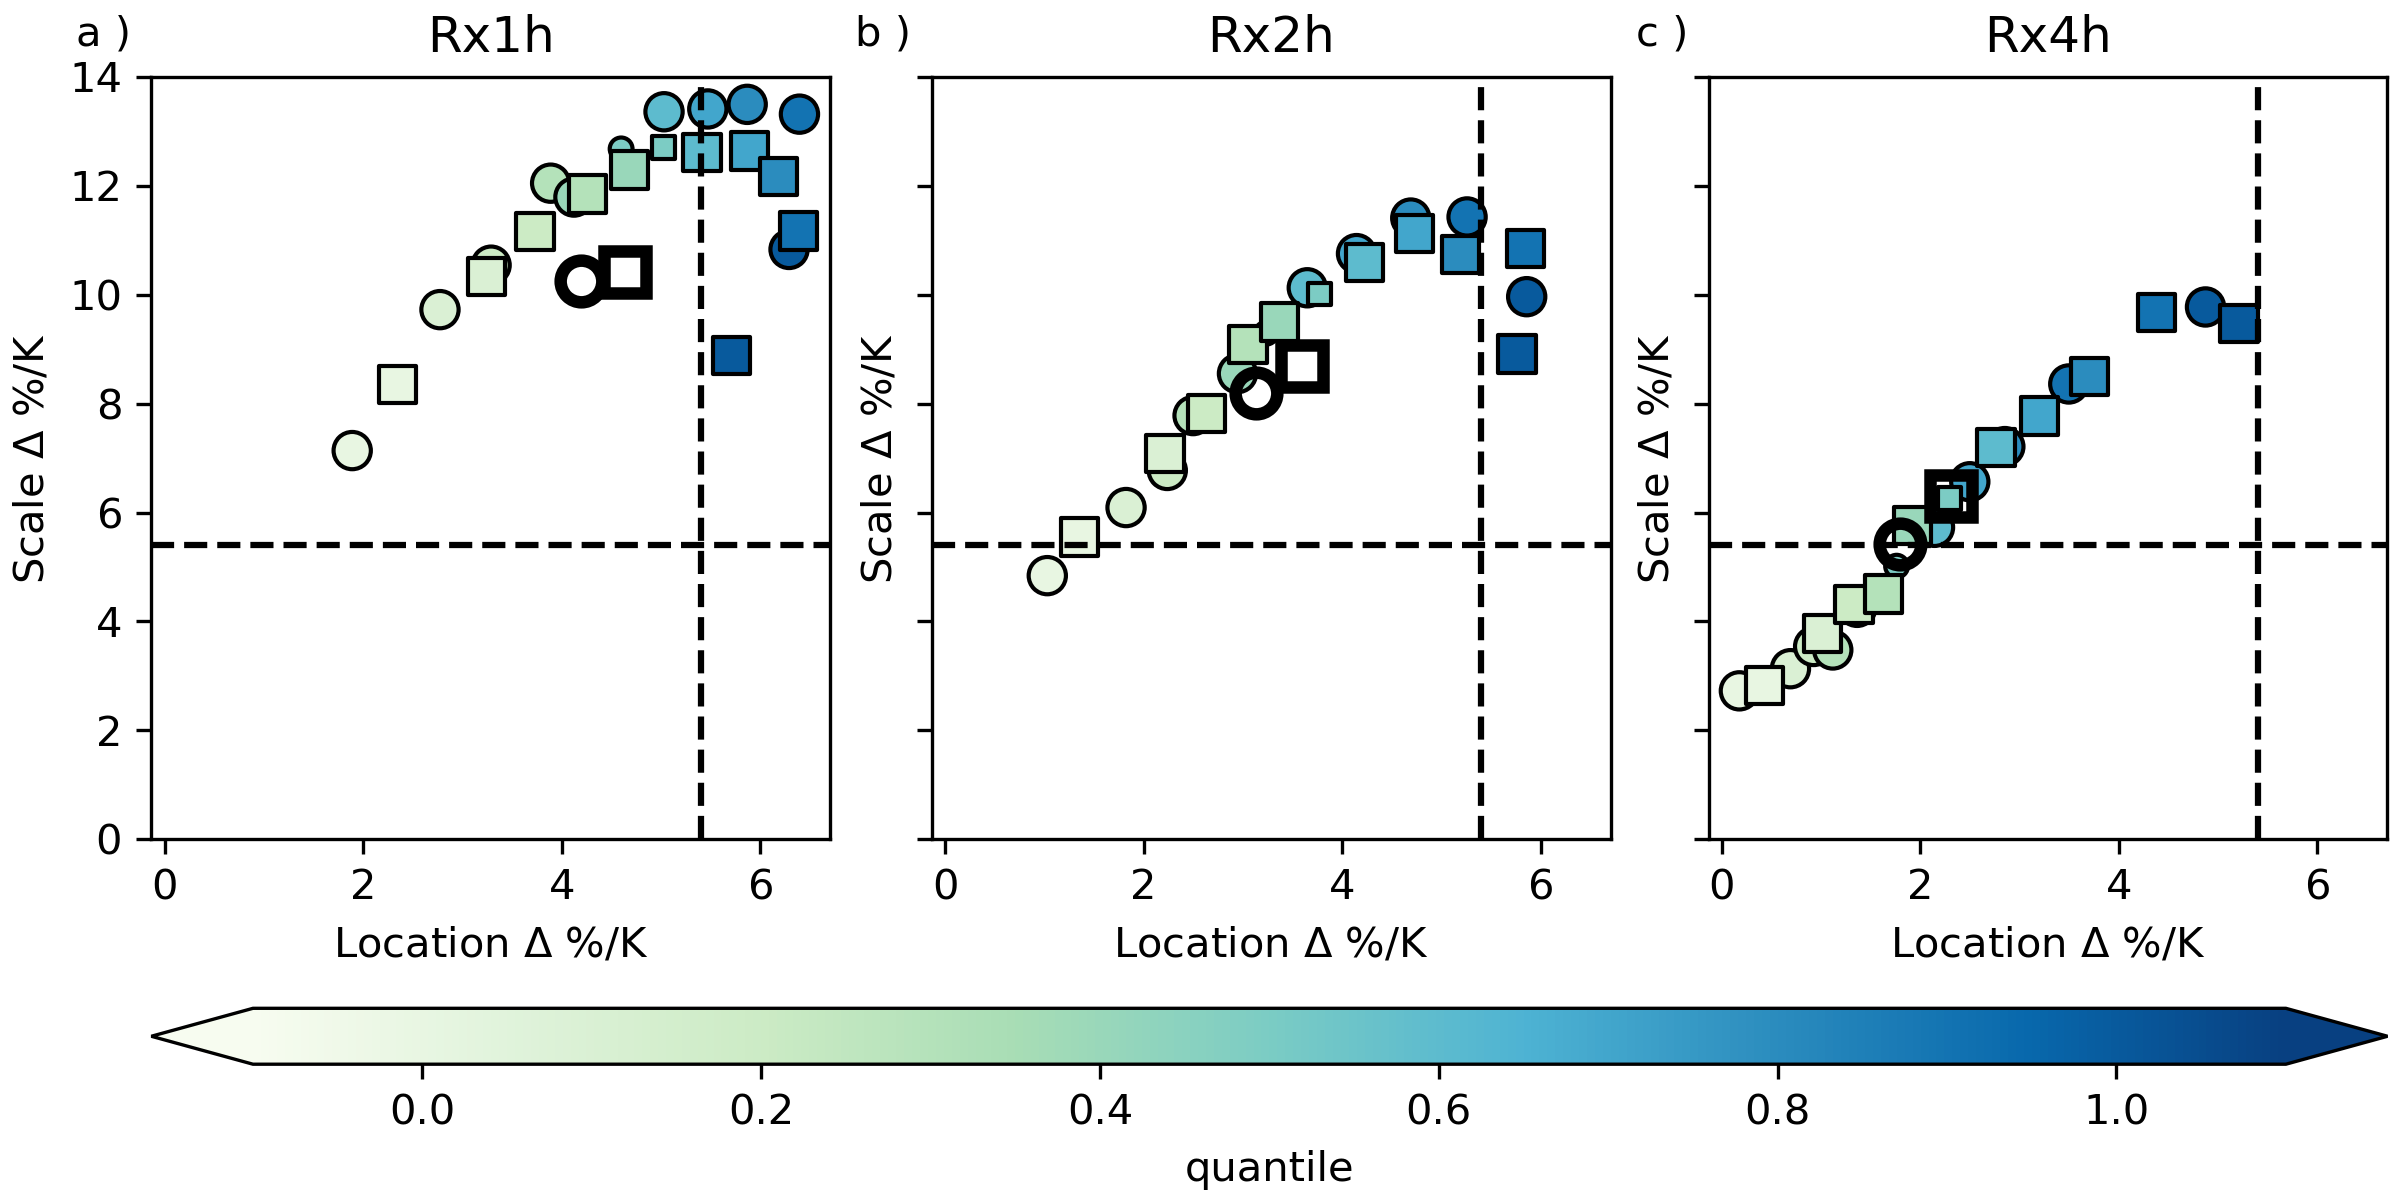
\includegraphics[width=\linewidth]{carmont_gev_quant_change}
%	\caption{
%		Fractional change in GEV scale  and location parameters for raw (purple) and filtered (black) CPM data. 
%				Numbers denote quantiles/10 in a 5x5 region (approximately 22x22 km) centred on Carmont Drain. Error bars are shown for the filtered rainfall data and are $2 \sigma$ differences  for each quantile relative to the whole region fit. 
%				Small numbers show where change is not significantly different from those of the whole region.
%				Dashed (red) horizontal and vertical lines show mean (double) Clausius-Clapeyron changes.
%				Circles show fractional change for the whole region.  Solid black line with x shows mean + 2 sigma change from shuffled CET fit values while dashed line shows same for mean values. 
%				Shown are Rx1h (a), Rx2h (b) and Rx4h values (c).
%	}
%	\label{fig:carmont_gev_quant_change}
%\end{figure}
%\clearpage
\begin{figure}[h!]
	\centering
	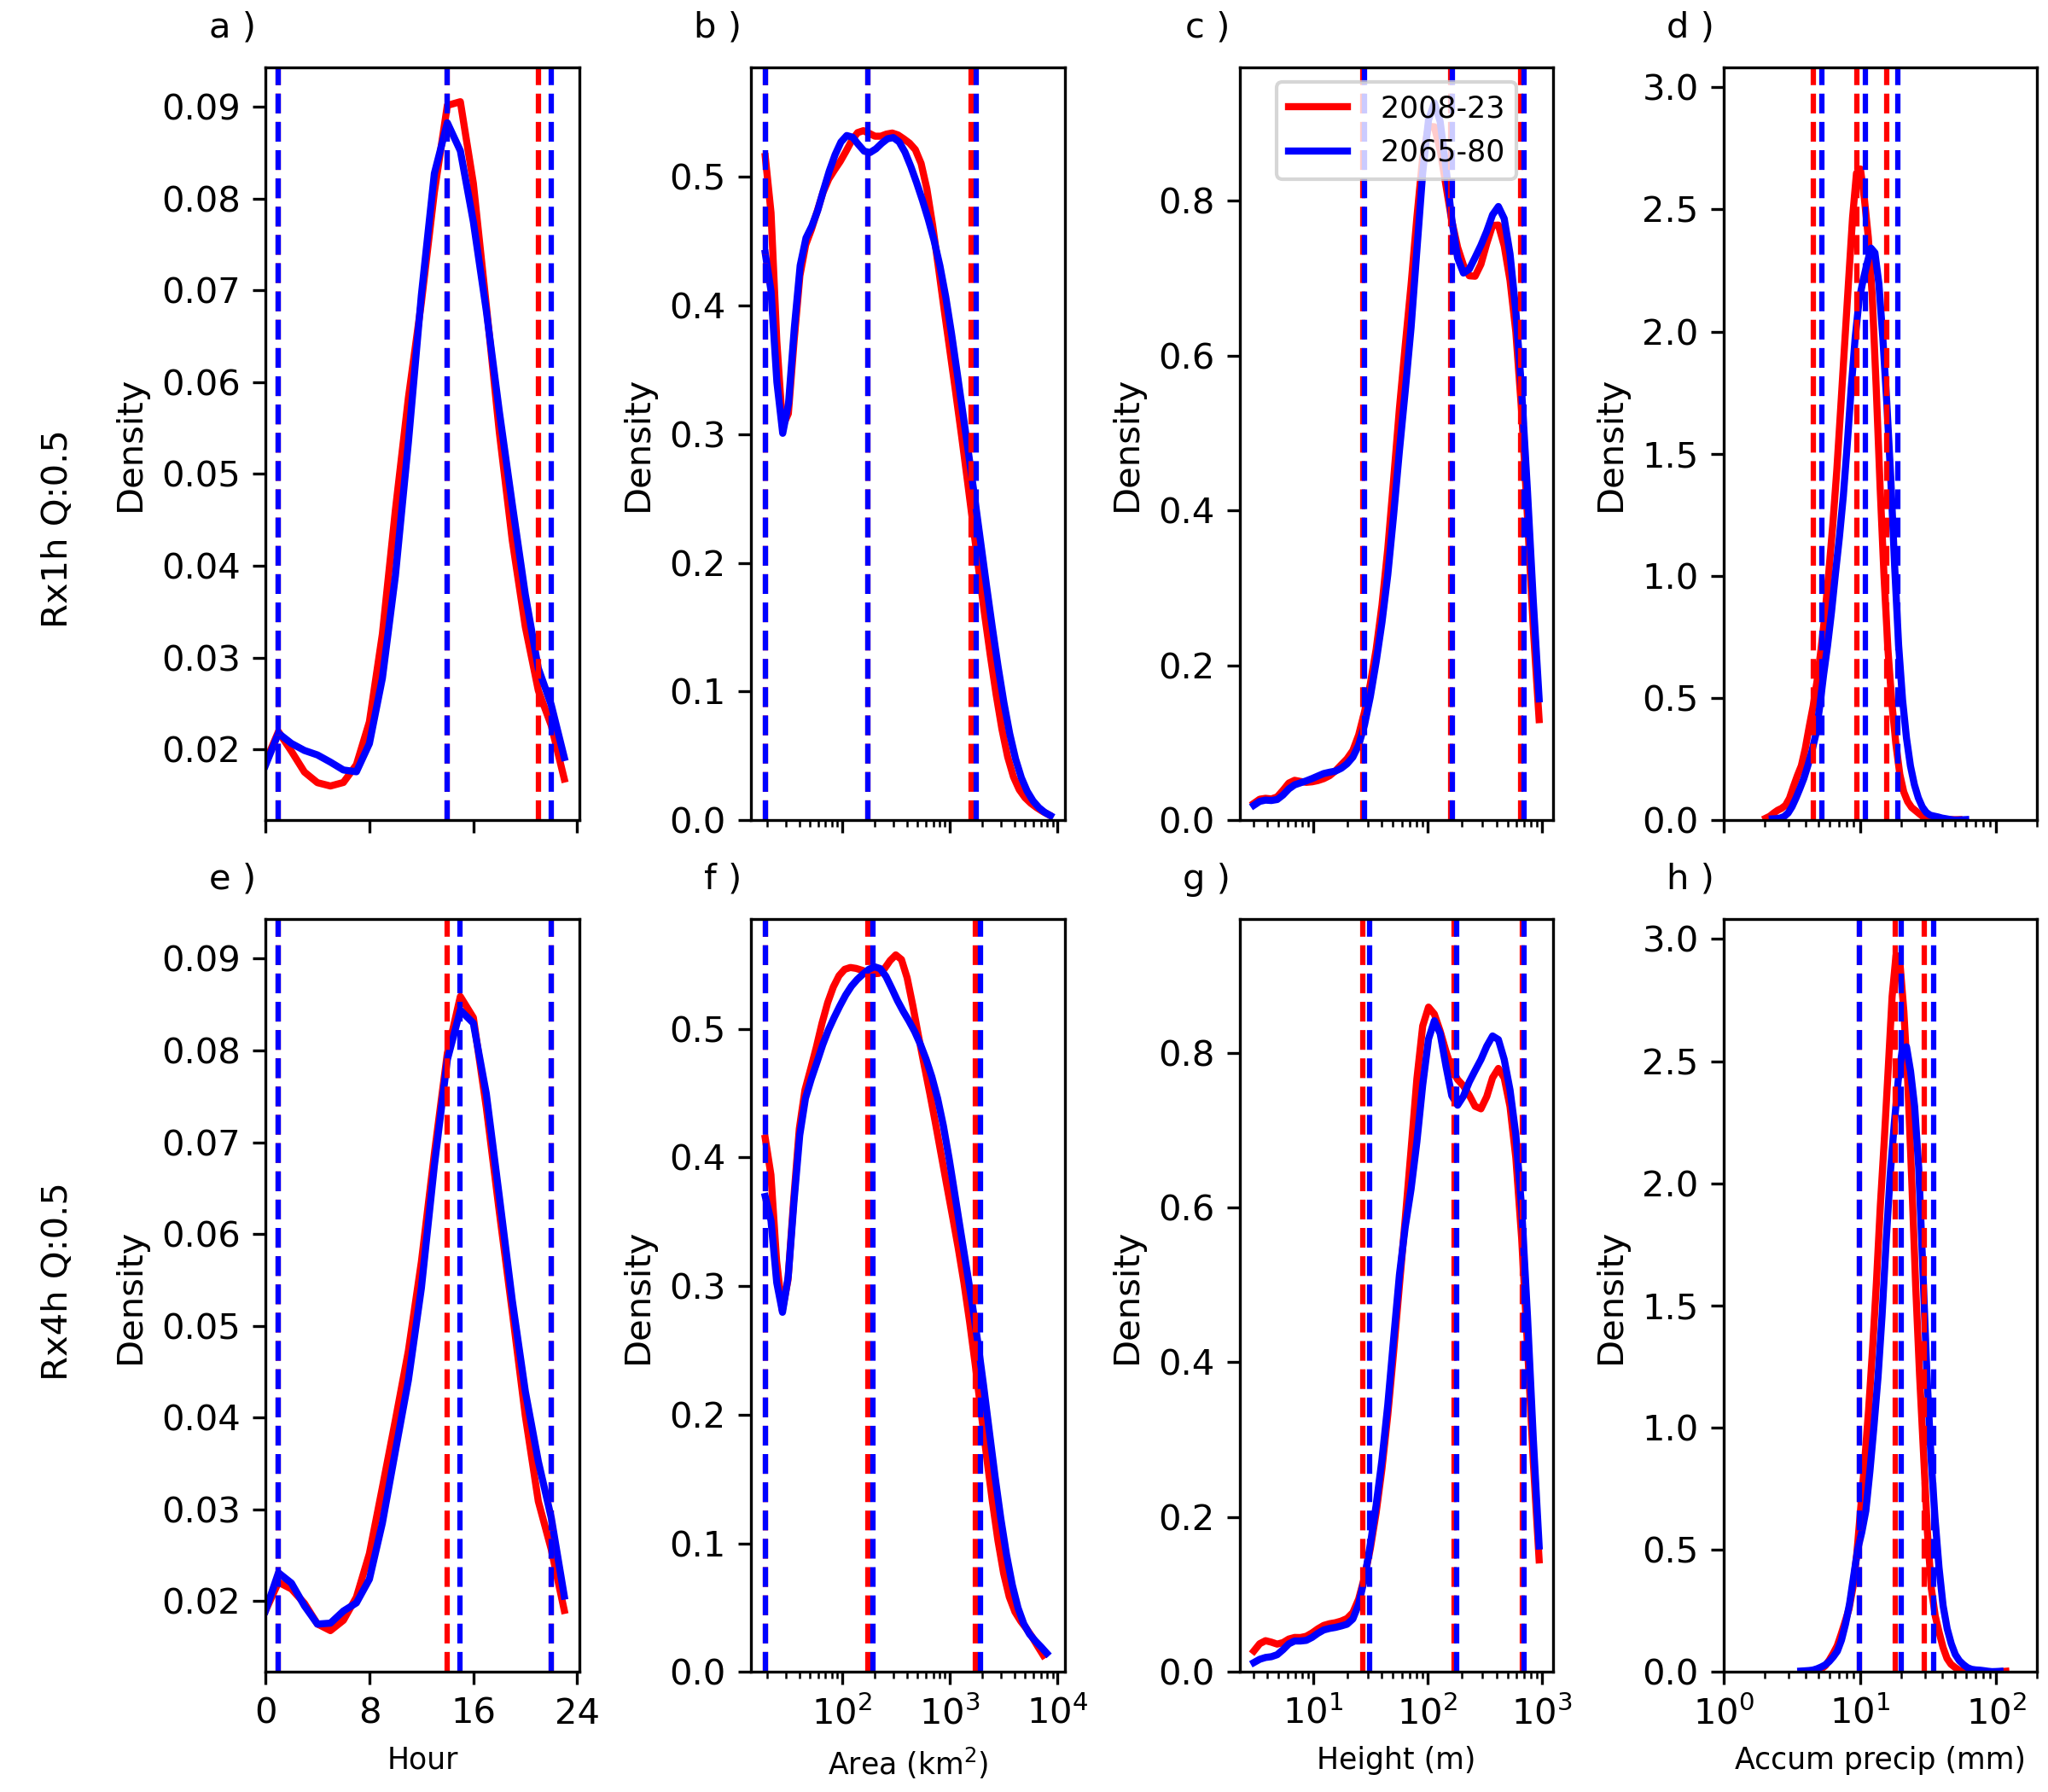
\includegraphics[width=\linewidth]{kde_smooth_events_2065_2080}
	\caption{a)-h): As figure~\ref{fig:kde_smooth_events} but only CPM data is shown for 2008-2023 (red) and 2065-2080 (blue) periods. Vertical dashed lines show 10, 50 and 90\% quantiles. Titles show variable with mean, or \%, increase for 2065-2080 relative to 2008-2023. i): \% increase (y-axis) in simulated event extreme precipitation, as a function of quantile within each event (x-axis), for 2065-2080 relative to 2008-2023 for Rx1h (solid) and Rx4h (dashed). All data is from filtered CPM data. }
	\label{fig:kde_smooth_events_2065_2080}
\end{figure}
%\pagebreak
%\appendix
%\renewcommand\thefigure{\thesection.\arabic{figure}}    
%\setcounter{figure}{0}  
%\section{Supp Figures}
%\FloatBarrier



\end{document}
